\pdfoutput=1
\documentclass[10pt,twocolumn,letterpaper]{article}
\usepackage[T1]{fontenc}
\usepackage[pagenumbers]{cvpr}
\usepackage{array,tabularx,multirow,microtype}
\definecolor{gaingreen}{HTML}{2A9D8F}
\newcommand{\gain}[1]{\,{\scriptsize\textcolor{gaingreen}{#1}}}  %
\newcommand{\ngr}{NGR}
\newcommand{\ls}{NGRR-LS}
\providecommand{\supp}[1]{Supp.~#1}  %
\providecommand{\main}[1]{main paper #1}  %

\usepackage{placeins}
\definecolor{cvprblue}{rgb}{0.21,0.49,0.74}
\usepackage[pagebackref,breaklinks,colorlinks,allcolors=cvprblue]{hyperref}
\title{Nucleate, Grow, Refine, Release: A Chemical-Process Framework for Robust Point Cloud Registration}
\author{Chengrui Xu$^{\dagger}$ \qquad Siyuan Jiang$^{\dagger}$ \qquad Xiaonan Wang$^{*}$\\
Tsinghua University\\
{\small $^{\dagger}$Equal contribution \qquad $^{*}$Corresponding author}\\
{\small Code and project page: \url{https://siyuanj.github.io/NGRR}}}
\begin{document}
\twocolumn[{%
\renewcommand\twocolumn[1][]{#1}%
\maketitle
\begingroup
\centering
\captionsetup{type=figure}
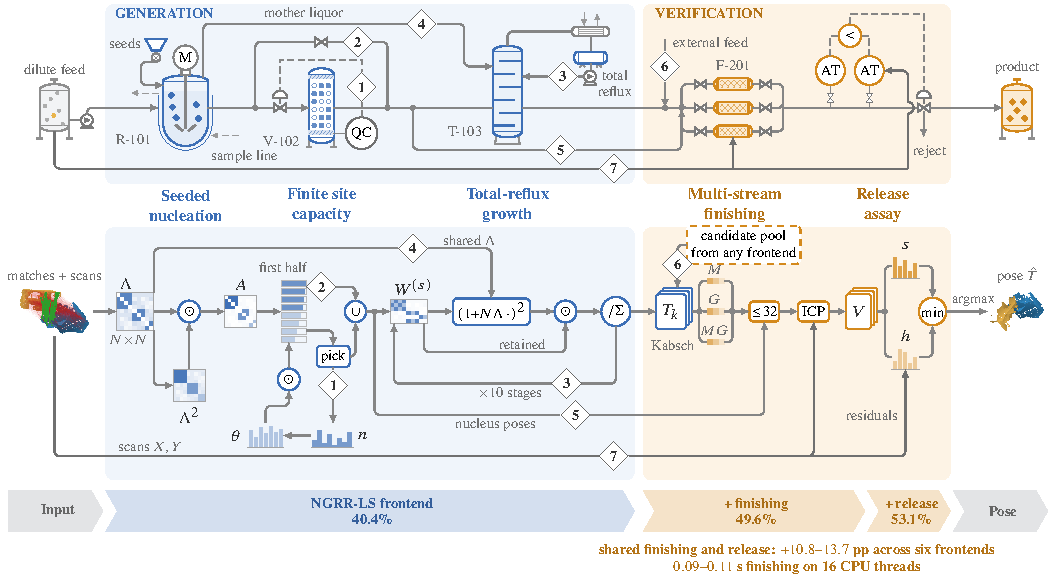
\includegraphics[width=\textwidth]{shared/figures/fig_dataflow.pdf}
\captionof{figure}{The chemical process (top) and registration data flow (bottom). NGRR-LS supplies one candidate pool, while the dashed entry makes the finishing and release backend available to any frontend. The compatibility matrix $\Lambda$ is used to generate hypotheses, which finishing turns into a refined pool $V$. Its candidates are evaluated by support $s$ and residual shape $h$. Release selects $\arg\max_k\min(s_k,h_k)$, corresponding to the low-signal selector over two analyzers. Diamonds 1--7 identify corresponding connections, including 3 for growth stages and total reflux and 7 for scans and the sample line. The bottom strip reports \ls{} recall on 3DLoMatch+FPFH after each stage. The refined-pool ceiling is 59.2\%. Scans are real, while matrices and equipment are schematic.}
\label{fig:flowsheet}
\endgroup%

\par\vspace{8pt}\noindent\makebox[\columnwidth][c]{\large\bfseries Abstract}\par
\vspace*{12pt}
}]

\begingroup
\renewcommand{\abstract}{\iftoggle{cvprpagenumbers}{}{\thispagestyle{empty}}\noindent\it\ignorespaces}
\renewcommand{\endabstract}{\par\vspace*{12pt}}
\begin{abstract}
Point cloud registration can fail even when a frontend has generated useful hypotheses. We introduce a training-free finishing and release backend for candidate pools from multiple frontends. Multi-stream finishing allocates a fixed surface-refinement budget using correspondence support, surface agreement and geometric information. Release combines geometric support with residual concentration. NGRR-LS complements this backend with a chemical-process-inspired generator: motif nucleation, finite site capacity and retained-composition growth preserve useful candidates. On all 1781 3DLoMatch+FPFH pairs, the same backend improves six frontends by 10.8 to 13.7 percentage points. Finishing takes 0.09 to 0.11 seconds with 16 CPU threads. With compiled NGRR-LS, the pipeline reaches 53.1\% recall in 0.39 seconds. Controls with the same ICP and release rule isolate candidate allocation, while coverage--selection diagnostics distinguish recovery from final selection. These results support viewing robust registration as a budget-constrained process of recovering refinable hypotheses and converting them into a reliable final pose.
\end{abstract}

\endgroup
\section{Introduction}
\label{sec:intro}

Point cloud registration estimates the rigid motion between two scans. Correspondence-based methods match local descriptors and then estimate the motion robustly from the putative matches. At low overlap, most of these matches are wrong: with FPFH~\cite{rusu2009fpfh} on 3DLoMatch~\cite{huang2021predator}, 888 of the 1781 pairs have fewer than 1\% correct matches (\cref{fig:dilute}). Robust estimators such as RANSAC~\cite{fischler1981ransac}, SC$^2$-PCR~\cite{chen2022sc2}, MAC~\cite{zhang2023mac} and TurboReg~\cite{yan2025turboreg} generate many pose hypotheses in this setting, but each returns only one of them.

A wrong output does not mean that every hypothesis is wrong. The six frontends we evaluate register 35.1 to 40.4\% of the 3DLoMatch+FPFH pairs natively (\cref{tab:main}). After up to 32 of their hypotheses are refined on the observed surfaces, a correct pose is present for 54.2 to 59.8\% of the pairs (\cref{tab:joint}). Each frontend thus loses 16.1 to 20.8 percentage points between its refined pool and its native output.

We therefore treat robust registration as two linked problems. \emph{Recovery} generates and preserves hypotheses that can be refined to the correct pose. \emph{Conversion} spends a limited refinement budget on these hypotheses and selects the final pose from the refined results. For conversion, we build a training-free backend that can follow any frontend. Multi-stream finishing allocates at most 32 point-to-plane ICP refinements across distinct candidates using correspondence support, surface agreement and geometric information. Release then selects from the refined pool by combining geometric support with the concentration of the residuals.

For recovery, we organize the generator after the unit operations that recover a scarce product in chemical separation~\cite{mccabe2005,mullin2001} (\cref{fig:flowsheet}). Each operation addresses one difficulty of generation from contaminated matches. Motif nucleation seeds candidate phases from compatible pairs or triples of matches. A finite site capacity, borrowed from adsorption, penalizes matches that many seeds already use, so that the seeds spread over several clusters. Growth that retains each phase's current composition, as in total reflux, enriches the phase with compatible matches. Together these operations form the NGRR-LS frontend. The analogy guides which operations the process contains, and we test each of them by removing or replacing it.

With the same settings for every frontend, the backend improves all six frontends by 10.8 to 13.7 percentage points on 3DLoMatch+FPFH, and its finishing stage takes 0.09 to 0.11\,s per pair on 16 CPU threads. With NGRR-LS, recall rises from 40.4\% for the native output to 49.6\% after finishing and 53.1\% after release, above the published results collected in \cref{tab:literature}. The compiled pipeline has a median time of 0.39\,s per pair, against 0.92\,s for SC$^2$-PCR with the same backend. Capacity raises the refined-pool coverage from 56.4\% to 59.2\% while native recall changes only from 40.3\% to 40.4\%, and the backend converts this coverage into a 2.0-point gain in final recall. With the same number of ICP calls on every frontend--input cell, finishing registers more pairs than a matched top-$K$ allocation (+693/$-$221 cells).

\paragraph{Contributions.} We make three contributions. (1) A training-free finishing and release backend that allocates a fixed surface-refinement budget across candidates and selects from the refined pool with complementary evidence. It improves six registration frontends at a finishing cost of 0.09 to 0.11\,s per pair. (2) The NGRR-LS frontend, which combines motif nucleation, soft site capacity and retained growth so that the pool contains a correct, refinable candidate more often. (3) An evaluation that separates candidate coverage from final selection, with stage diagnostics, interventions on each operation, controls at a matched ICP budget, nine real-data cohorts and CPU timing.

\section{Related work}
\label{sec:related}
\paragraph{Recovering hypotheses.} RANSAC and MLESAC sample minimal sets~\cite{fischler1981ransac,torr2000mlesac}. TEASER++, TriVoC and TEAR use robust estimation and geometric bounds~\cite{yang2021teaser,sun2022trivoc,huang2024tear}. Compatibility graphs support spectral matching~\cite{leordeanu2005spectral}, SC$^2$-PCR~\cite{chen2022sc2}, maximal-clique registration~\cite{zhang2023mac} and TurboReg~\cite{yan2025turboreg}. CG-SAC and SAC-COT rank compatible pairs and triangles~\cite{quan2020cgsac,yang2022saccot}. Multiplicative dynamics relate to dominant sets and game-theoretic matching~\cite{pavan2007dominant,albarelli2010game}. Our generator builds on these structures with independently seeded phases that retain their composition and a cumulative occupancy penalty that distributes the nucleus budget.

\paragraph{Refining and verifying candidates.} SC$^2$-PCR generates seed-wise transformations, ranks them by correspondence support and refines the selected estimate~\cite{chen2022sc2}. MAC extracts local consensus through maximal cliques and estimates transformations for its selected cliques~\cite{zhang2023mac}. Surface hypothesis verification~\cite{aldoma2012ghv}, point-to-plane ICP~\cite{besl1992icp,chen1992medioni} and geometrically informed sampling~\cite{gelfand2003stable} supply complementary tools. SC$^2$-PCR++ revisits generation and selection~\cite{chen2023sc2pp}. MAC1toK expands matching candidates~\cite{zhang2026mac1tok}, and Regor and DualReg exploit point clouds beyond the initial matches~\cite{zhao2025regor,li2026dualreg}.

Our verification stages decide which candidates receive refinement and how the refined poses are compared. Finishing distributes the refinement budget over distinct pose modes using several evidence rankings and a non-dominated frontier. Release uses both geometric support and residual concentration to assess the extent and quality of alignment. We apply these stages to each frontend's pool and native output using the same settings.

\paragraph{Diversity and process-inspired design.} Maximal marginal relevance (MMR)~\cite{carbonell1998mmr} and suppression balance relevance and redundancy. Site capacity applies a soft, cumulative penalty to reused matches. A same-budget comparison places it within this family (\cref{sec:crowding}). Physics-inspired computation can transfer a dynamical rule, as in simulated annealing~\cite{kirkpatrick1983annealing}. The chemical-process view organizes recovery, enrichment, finishing and release by their constraints and failure mechanisms. We test their roles through interventions on each operation.

\section{Registration as a separation process}
\label{sec:method}

Given $N$ putative matches $(p_i,q_i)\in\mathbb R^3\times\mathbb R^3$ and observed clouds $X,Y$, we seek a rigid transform $(R,t)$. In \cref{fig:flowsheet}, recovery generates and preserves pose hypotheses, while conversion allocates refinement and selects the final pose. The operations share a candidate pool and its geometric evidence, with a separate budget or decision criterion at each stage. Full implementation details are in \supp{\cref*{S-sec:s-method}}.

\subsection{Seeded nucleation}
\label{sec:nucleation}

With one correct match in a hundred, a uniform initialization places most of its mass on outliers. We initialize candidate phases from geometric motifs, following the use of seed crystals to initiate crystallization in a dilute solution. The zero-diagonal compatibility graph is
\begin{equation}
\Lambda_{ij}=\exp\!\Big(-\frac{(\|p_i-p_j\|-\|q_i-q_j\|)^2}{2\sigma_c^2}\Big),\qquad i\neq j.
\label{eq:compat}
\end{equation}
Here $\sigma_c=0.375\tau$, with the distance scale $\tau$ of \cref{sec:finishing}. Pairs are ranked by the second-order compatibility $\Lambda_{ab}(\Lambda^2)_{ab}$~\cite{chen2022sc2} and triples by $T_{abc}=\Lambda_{ab}\Lambda_{bc}\Lambda_{ca}\sum_d\Lambda_{ad}\Lambda_{bd}\Lambda_{cd}$. Each selected motif initializes one phase, a probability vector over all matches, $w^{(0)}_i\propto\delta_{ia}+\delta_{ib}+\Lambda_{ai}\Lambda_{bi}$ for a pair $(a,b)$ and analogously for a triple (\supp{\cref*{S-sec:s-method}}). A background-load scheduler uses 256 pair seeds when $(N-2)\bar\Lambda^2<1$, where $\bar\Lambda$ is the mean off-diagonal compatibility, a background-support proxy below one under an independent-edge approximation. Otherwise it extends a shortlist of 4096 pairs to $K=1024$ triples. All $K$ phases evolve independently.

\subsection{Finite site capacity}
\label{sec:capacity}

A cluster of $n$ mutually compatible wrong matches contains $\binom{n}{2}$ internal pairs, each supported by about $n-2$ triangles. Among $m$ true inliers, a true pair collects about $m-2$, only 8 to 23 for the 10 to 25 inliers typical of hard pairs. Ranking by compatibility alone can therefore fill most seed slots with motifs from a few incorrect clusters (\cref{sec:crowding}).

Finite adsorption capacity motivates a penalty on repeated use of each match~\cite{langmuir1918}. We assign match $x$ a site vacancy
\begin{equation}
\theta_x=\frac{1}{1+n_x/q},
\label{eq:vacancy}
\end{equation}
where $n_x$ counts the already selected motifs containing $x$. A motif's affinity is discounted by the vacancies of its matches, $T_{abc}\,\theta_a\theta_b\theta_c$ (pairs analogously). The first half of the pair shortlist and of the nuclei keep the original ranking. We fill the second half greedily by discounted affinity from a deeper ranking. Growth, fitting and scoring are unchanged. The resulting frontend is NGRR-LS, the generator of the NGRR framework (nucleate, grow, refine, release) with Langmuir site capacity. Without capacity, the same generator is NGR. The vacancy is a Langmuir-form occupancy feedback rule, not a derived adsorption equilibrium. We fixed its capacities, $q=8$ for pairs and $q=4$ for triples, at pre-registration and never tuned them. \Cref{sec:crowding} compares three alternatives. MMR~\cite{carbonell1998mmr} subtracts the largest overlap with any single selected motif. Hard capacity rejects a motif once one of its matches is held $q$ times. Pose NMS rejects a nucleus whose three-point pose repeats an earlier one.

\subsection{Total-reflux growth}
\label{sec:reflux}

Each phase undergoes ten updates:
\begin{equation}
w_i^{(s+1)}=\frac{w_i^{(s)}\,[\epsilon+N(\Lambda w^{(s)})_i]^{\beta}}{\sum_j w_j^{(s)}\,[\epsilon+N(\Lambda w^{(s)})_j]^{\beta}},\quad \epsilon=1,\ \beta=2.
\label{eq:growth}
\end{equation}
The factor $w_i^{(s)}$ retains the current composition when applying the support update. This follows the retention principle of total reflux, in which condensate is returned to the column. Growth can also reinforce a coherent incorrect cluster. Each grown phase gives a weighted Kabsch fit~\cite{kabsch1976}, refitted twice on matches whose residual $r_i$ is below a fixed radius $\tau_c=\tau$. The native winner maximizes the number of these matches with pair seeds, with a small mean-residual penalty (the \emph{count readout}) and $\sum_i[1-r_i/\tau_c]_+$ with triple seeds (the \emph{MAE readout}).

\subsection{Multi-stream finishing}
\label{sec:finishing}

Finishing distributes a limited refinement budget across pose hypotheses before final selection. Let $\mathcal H$ contain the frontend's candidate pool and native winner. Given the observed clouds, finishing allocates $A_B=\mathcal A_B(\mathcal H;X,Y)$, $|A_B|\le B$, and returns the valid refined pool
\begin{equation}
V=\{\mathcal R(T;X,Y):T\in A_B\},
\label{eq:conversion}
\end{equation}
where $\mathcal R$ is the fixed ICP procedure. Release selects from $V$. Allocation uses complementary evidence and pose diversity to avoid spending the budget on repeated poses. The frontend retains its native refinement.

We retain the native winner in a shortlist of at most 32 candidates separated by $5^\circ$ and $\tau$ in pose space. The shortlist ranks the frontend's stored hypotheses by $M$ alone, for example the best 2000 of RANSAC's $10^6$ trials. Full-query $G$ is evaluated on this shortlist and selected auxiliary candidates; the coarse $I$ screen can examine the entire raw and auxiliary pools. Up to 16 primary refinements are allocated by interleaving rankings of correspondence support $M$, surface support $G$, and $MG$. We then add distinct candidates from the non-dominated correspondence/information-support frontier, up to a total cap $B=32$. This retains candidates with different trade-offs between the two cues. NGR's direct nucleus poses enter the same allocation. Each selected pose undergoes two-scale point-to-plane ICP~\cite{besl1992icp,chen1992medioni} at $2\tau$ and $\tau$, with Tukey weights and at most ten iterations per scale. We use $\tau=0.1$\,m indoors, $0.3$\,m on ETH and $0.6$\,m on KITTI. Release adds no refinement.

Let $\kappa(r)=[1-r/\tau]_+$. Correspondence support is $M(T)=\sum_i\kappa(\|Rp_i+t-q_i\|)$. To compute surface support $G(T)$, we average $\kappa(d)$ in each nearest-neighbor direction between the clouds, then take the harmonic mean of these averages. Information support $I(T)$ uses the same construction with normalized leverage weights, computed once on each cloud's query points and independent of $T$,
\begin{equation}
a_x\propto j_x^\top(J^\top J)^\dagger j_x,\qquad
j_x=[(\widetilde x\times \nu_x)^\top,\nu_x^\top]^\top ,
\end{equation}
where $\widetilde x$ is centered and scale-normalized and $\nu_x$ is a surface normal~\cite{gelfand2003stable}. Leverage weights each query by its relative contribution to the point-to-plane constraints. Fitting uses a fixed random half of the source cloud, and surface queries use the other half of each cloud, at most 4096 points each.

For the finishing-only ablation, an anchor maximizes $M\sqrt G$ among primary refinements. A challenger is admitted if it improves $M\sqrt I$ without reducing $I$. The complete pipeline keeps the valid refined pool $V$ for release.

\subsection{Release assay}
\label{sec:assay}

A broad accidental alignment can have substantial support, while a small coherent patch can have concentrated residuals. Release therefore evaluates both the extent and the quality of agreement. For candidate $k$ in the refined pool $V$, the support channel is $s_k=M_k\sqrt{I_k}/\max_{j\in V}M_j\sqrt{I_j}$. The shape channel measures how tightly the supported queries lie on the other surface. For the $m$ query points whose nearest-neighbor distance $d$ is below $\tau$, let $u=d^2/\tau^2$ and $\bar u=\frac1m\sum u$. Under the idealized radial reference density $p_0(d)=2d/\tau^2$ on $[0,\tau)$, $\Pr(d\le r\mid d<\tau)=r^2/\tau^2$, so $u$ is uniform on $[0,1)$ and $\bar u\approx\frac12$. The Cram\'er rate of a smaller mean under this null,
\begin{equation}
\psi(\bar u)=\sup_{\beta\ge0}\Big\{-\beta\bar u-\log\frac{1-e^{-\beta}}{\beta}\Big\},
\label{eq:psi}
\end{equation}
is the per-point evidence that the residuals concentrate near zero. It is zero for $\bar u\ge\frac12$. Averaging $\psi$ over the two directions gives $J_k$, and $h_k=\exp(J_k-\max_{j\in V}J_j)$. Release selects
\begin{equation}
\hat k=\arg\max_{k\in V}\ \min\{s_k,\,h_k\},
\label{eq:assay}
\end{equation}
breaking ties by $s_k$, then $h_k$, then queue order. The weaker normalized channel determines each candidate's score, so a high score requires both specifications. This rule ranks candidates within $V$ without fitting a mixing weight.

For nondegenerate normalized channels, consider the surrogate utility $\lambda s_k+(1-\lambda)h_k$ for an unknown exchange rate $\lambda\in[0,1]$. The regret of choosing $k$ is convex in $\lambda$, so its maximum over $\lambda$ lies at an endpoint. Since both channels are normalized to a maximum of one, this maximum is $\max\{1-s_k,1-h_k\}$. Minimizing worst-case regret therefore gives \cref{eq:assay}. \Cref{sec:verification} evaluates the resulting ranking and decision rule on real scans.

A conditional logit can instead select among the candidates of a pool. It uses 26 label-free features of the finishing quantities and is trained only on the 3DMatch training scenes. We report this learned variant separately from the training-free results.

\phantomsection\label{sec:diagnosis}
To separate recovery from final selection, let $z_\ell$ indicate whether refined pool $V_\ell$ contains a correct pose and $y_\ell$ whether release selects one. Over $L$ pairs,
\begin{equation}
C=\frac{\sum_\ell z_\ell}{L},\quad R=\frac{\sum_\ell y_\ell}{L},\quad E=\frac{\sum_\ell y_\ell}{\sum_\ell z_\ell},\qquad R=CE.
\label{eq:coverage}
\end{equation}
Set $E=0$ if no pair is covered. Coverage depends on generation and the specified refinement, so we hold finishing fixed when comparing generators. Holding the refined pool fixed isolates release.

\section{Experiments}
\label{sec:experiments}

\paragraph{Data and protocol.}\label{sec:protocol} We evaluate nine cohorts. 3DMatch (1623 pairs) and 3DLoMatch (1781 pairs) use FPFH, FCGF and GeoTransformer correspondences~\cite{zeng2017match,huang2021predator,rusu2009fpfh,choy2019fcgf,qin2022geotransformer}. KITTI has 555 pairs with FPFH and FCGF~\cite{geiger2012kitti}, and ETH has 713 pairs with FPFH~\cite{pomerleau2012eth}. Each input has at most 5000 matches. Success requires RE $\le15^\circ$ and TE $\le0.3$\,m indoors. On KITTI, it requires RE $\le5^\circ$ and TE $\le0.6$\,m. On ETH, it requires RE $<2^\circ$ and TE $<0.3$\,m. GeoTransformer's official scene-mean criterion is reported separately.

Capacity and release were pre-registered, with adoption decisions on 3000 pairs from 82 disjoint 3DMatch training scenes. Public-benchmark evaluations informed the earlier NGR and finishing designs, so those benchmarks were not held out during their development. A registered budget-filling extension was evaluated once on test data and omitted after negligible final gains. The supplementary material discloses that decision and the optional learned release. ETH was not used for algorithm-adoption decisions. Comparisons use paired tests; Holm-adjusted values are labelled.

\paragraph{Controlled comparison.} RANSAC-1M, SC$^2$-PCR, MAC, TurboReg, NGR and NGRR-LS use the same correspondences, each retaining its candidate generation and native refinement. The verification stages supply identical surfaces, allocation, ICP settings, scoring and at most 32 refinements. SC$^2$-PCR and MAC use their authors' code, and TurboReg its author core.

\subsection{Overall performance and cross-frontend \texorpdfstring{\mbox{transfer}}{transfer}}
\label{sec:product}


\begin{table}[t]
\caption{Stage diagnosis on 1781 LoMatch+FPFH pairs. Gains (pp) compare winner ICP with native output, finishing with winner ICP, and release with finishing. $C$: correct refined-pose coverage; $E$: correct selection among covered pairs. Final accuracy and time are in \cref{tab:main}.}
\label{tab:joint}
\centering
\small\setlength{\tabcolsep}{3.5pt}
\begin{tabular}{@{}lrrrrr@{}}
\toprule
 & \multicolumn{3}{c}{Stage gains (pp)} & \multicolumn{2}{c}{Pool (\%)} \\
\cmidrule(lr){2-4}\cmidrule(l){5-6}
Frontend & $\Delta$ICP & $\Delta$Finish & $\Delta$Release & $C$ & $E$ \\
\midrule
RANSAC-1M & +4.77 & +5.84 & +3.09 & 54.2 & 90.1 \\
SC$^2$-PCR & +3.26 & +7.47 & +2.86 & 59.8 & 87.9 \\
MAC (C++) & +3.20 & +6.18 & +2.25 & 59.7 & 86.4 \\
TurboReg & +3.31 & +7.24 & +2.53 & 56.4 & 91.3 \\
NGR & +2.58 & +5.84 & +2.41 & 56.4 & 90.6 \\
NGRR-LS & +2.58 & +6.63 & +3.48 & 59.2 & 89.8 \\
\bottomrule
\end{tabular}

\end{table}

\Cref{tab:joint} diagnoses the successive stages of the common backend, while \cref{tab:main} compares final accuracy, pose errors and runtime. The backend improves the six original frontends by 10.8 to 13.7 percentage points on 3DLoMatch+FPFH. Refining only each native winner accounts for 2.6 to 4.8 of these points, and multi-candidate finishing and release add the remaining 8.3 to 10.3. The backend's finishing stage takes 0.09 to 0.11\,s in the 16-thread timing setting. NGRR-LS improves from 40.4\% to 53.1\% with FPFH and from 59.2\% to 66.7\% with FCGF. These gains hold for frontends based on random sampling, spectral or compatibility scores, cliques and seeded growth.

With this backend fixed, NGRR-LS reaches 53.1\% recall, compared with 52.6\% for SC$^2$-PCR and 51.6\% for MAC. The paired difference between NGRR-LS and SC$^2$-PCR is not statistically significant (+42/$-$32, raw $p=0.30$). Their reported median registration-stage times are 0.39\,s and 0.92\,s, respectively. Compiled NGRR-LS therefore has a 57.2\% lower measured median time on the common timing subset. The paired comparison with MAC is +55/$-$28 (raw $p=0.004$), and the paired comparison with NGR is +45/$-$9. Starting from the same correspondences, SC$^2$-PCR++~\cite{chen2023sc2pp}, Regor~\cite{zhao2025regor} and DualReg~\cite{li2026dualreg} natively reach 43.9, 45.3 and 37.4\% (\cref{tab:main}). Across all nine cohorts, the five frontends evaluated on all nine cohorts register 9771 to 9948 of 12\,035 pairs, and NGRR-LS registers 9920. On 3DLoMatch+FPFH, the scene bootstrap gives a 12.7 [10.3,14.1] percentage-point gain over the native output and a 2.0 [1.5,2.5] percentage-point gain over NGR. Its difference from SC$^2$-PCR is 0.6 [$-0.3$,1.6] percentage points (\supp{\cref*{S-sec:s-results}}).

\begin{table*}[t]
\caption{Controlled-input performance (first $\le5000$ matches). RR in \%; RE ($^\circ$) and TE (cm) are means over each row's successful pairs. F+R: common finishing and release. Bold/underline: best/second RR within native or F+R rows. Time: median registration stage on 100 LoMatch+FPFH pairs, EPYC 9655P CPU (16 threads; MAC 12), except Regor (GPU); loading/features excluded. $^\dagger$: GPU accuracy, separate CPU timing. -- denotes unavailable settings. SC$^2$-PCR++ and Regor additionally use descriptors; Regor re-matches, and DualReg uses estimated normals. Protocols and timing: Supp.~Sec.~\ref*{S-sec:s-results}.}
\label{tab:main}
\centering\fontsize{8}{9}\selectfont\setlength{\tabcolsep}{1.35pt}
\begin{tabular}{@{}lccccccccccccccccccc@{}}
\toprule
 & \multicolumn{6}{c}{3DMatch} & \multicolumn{6}{c}{3DLoMatch} & \multicolumn{6}{c}{KITTI} & Time (s) \\
\cmidrule(lr){2-7}\cmidrule(lr){8-13}\cmidrule(lr){14-19}
 & \multicolumn{3}{c}{FPFH} & \multicolumn{3}{c}{FCGF} & \multicolumn{3}{c}{FPFH} & \multicolumn{3}{c}{FCGF} & \multicolumn{3}{c}{FPFH} & \multicolumn{3}{c}{FCGF} & 3DLM \\
\cmidrule(lr){2-4}\cmidrule(lr){5-7}\cmidrule(lr){8-10}\cmidrule(lr){11-13}\cmidrule(lr){14-16}\cmidrule(lr){17-19}
Method & RR & RE & TE & RR & RE & TE & RR & RE & TE & RR & RE & TE & RR & RE & TE & RR & RE & TE & FPFH \\
\midrule
\multicolumn{20}{@{}l}{\emph{Correspondence frontends (C++ MAC also uses clouds to set its distance scale)}} \\
RANSAC-1M & 82.32 & 2.40 & 7.13 & 92.48 & 2.20 & 6.74 & 35.09 & 4.14 & 10.57 & 57.94 & 3.85 & 10.80 & \underline{99.64} & 0.36 & 8.25 & \underline{97.30} & 0.31 & 21.38 & 0.44 \\
SC$^2$-PCR & 83.67 & 2.19 & 6.79 & 92.91 & 2.10 & 6.51 & 38.97 & 3.96 & 10.41 & 58.28 & 3.58 & 10.42 & 99.46 & 0.30 & 6.56 & 95.86 & 0.31 & 20.01 & 0.83 \\
MAC & 82.99 & 2.12 & 6.63 & 93.47 & 2.08 & 6.49 & 39.98 & 3.77 & 10.17 & 59.01 & 3.52 & 10.32 & \underline{99.64} & 0.29 & 6.71 & 95.68 & 0.30 & 20.12 & 1.55 \\
TurboReg & 83.73 & 2.24 & 6.80 & 93.35 & 2.08 & 6.47 & 38.46 & 3.89 & 10.21 & 58.67 & 3.58 & 10.35 & \textbf{99.82} & 0.30 & 6.46 & 95.50 & 0.30 & 19.94 & 1.84 \\
NGR & 83.36 & 2.13 & 6.63 & 92.85 & 2.07 & 6.42 & 40.26 & 3.79 & 10.21 & 58.96 & 3.57 & 10.37 & \textbf{99.82} & 0.31 & 6.96 & 95.32 & 0.31 & 19.73 & 0.29 \\
NGRR-LS & 83.43 & 2.13 & 6.64 & 93.16 & 2.06 & 6.41 & 40.43 & 3.81 & 10.21 & 59.24 & 3.56 & 10.34 & \underline{99.64} & 0.31 & 7.12 & 95.32 & 0.31 & 19.72 & 0.30 \\
\midrule
\multicolumn{20}{@{}l}{\emph{Using the point clouds}} \\
SC$^2$-PCR++$^\dagger$ & \underline{87.86} & 2.16 & 6.69 & \underline{93.72} & 2.10 & 6.50 & \underline{43.85} & 3.83 & 10.35 & \underline{60.42} & 3.53 & 10.41 & \textbf{99.82} & 0.33 & 7.33 & \textbf{98.20} & 0.33 & 21.13 & 0.71 \\
Regor & \textbf{88.91} & 1.70 & 5.93 & \textbf{94.15} & 1.80 & 6.10 & \textbf{45.26} & 2.91 & 9.26 & \textbf{61.31} & 2.95 & 9.43 & -- & -- & -- & -- & -- & -- & 0.11 GPU \\
DualReg & 82.07 & 1.84 & 6.21 & 92.73 & 1.83 & 6.39 & 37.39 & 3.15 & 9.40 & 58.28 & 3.06 & 9.83 & 94.05 & 0.25 & 7.52 & 93.51 & 0.26 & 18.54 & 0.09 \\
\midrule
\multicolumn{20}{@{}l}{\emph{Each frontend + our common finishing and release (F+R)}} \\
RANSAC-1M + F+R & 90.20 & 1.57 & 5.96 & \textbf{94.89} & 1.60 & 6.09 & 48.79 & 2.53 & 8.96 & \textbf{67.10} & 2.55 & 9.21 & \textbf{99.82} & 0.13 & 3.55 & \textbf{99.46} & 0.12 & 3.43 & 0.54 \\
SC$^2$-PCR + F+R & \textbf{91.00} & 1.58 & 5.98 & \textbf{94.89} & 1.61 & 6.12 & \underline{52.55} & 2.56 & 8.96 & \underline{66.98} & 2.56 & 9.18 & \textbf{99.82} & 0.13 & 3.55 & \underline{99.28} & 0.13 & 3.64 & 0.92 \\
MAC + F+R & 90.45 & 1.56 & 5.94 & \underline{94.76} & 1.61 & 6.10 & 51.60 & 2.55 & 8.82 & 66.37 & 2.54 & 9.16 & \textbf{99.82} & 0.13 & 3.56 & 98.92 & 0.12 & 3.55 & 1.68 \\
TurboReg + F+R & 90.39 & 1.57 & 5.98 & \underline{94.76} & 1.61 & 6.10 & 51.54 & 2.50 & 8.89 & 66.09 & 2.54 & 9.18 & \textbf{99.82} & 0.14 & 3.54 & \textbf{99.46} & 0.13 & 3.67 & 1.96 \\
NGR + F+R & 90.33 & 1.58 & 5.99 & 94.45 & 1.61 & 6.11 & 51.09 & 2.54 & 8.96 & 65.69 & 2.57 & 9.30 & \textbf{99.82} & 0.13 & 3.57 & \underline{99.28} & 0.12 & 3.41 & 0.38 \\
NGRR-LS + F+R & \underline{90.51} & 1.57 & 5.95 & \textbf{94.89} & 1.61 & 6.14 & \textbf{53.12} & 2.54 & 8.99 & 66.70 & 2.55 & 9.23 & \textbf{99.82} & 0.13 & 3.57 & \textbf{99.46} & 0.12 & 3.44 & 0.39 \\
\bottomrule
\end{tabular}

\end{table*}

\begin{figure*}[t]
\centering
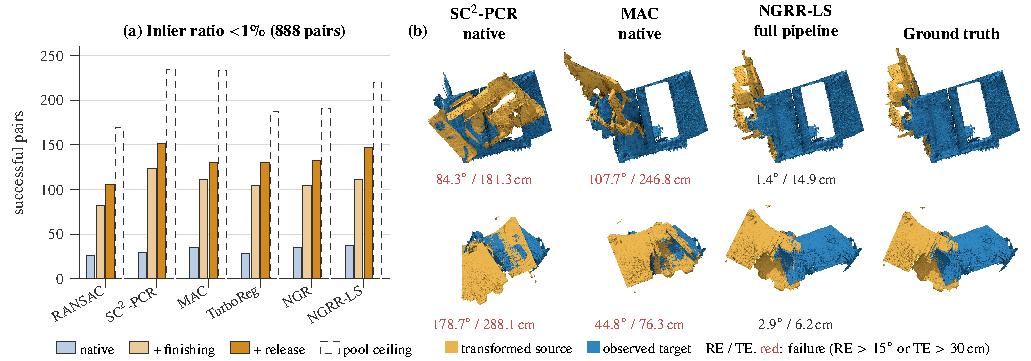
\includegraphics[width=\textwidth]{figures/fig_dilute.pdf}
\caption{(a) All 888 3DLoMatch+FPFH pairs below 1\% inliers: native, finishing, release and refined-pool ceiling. (b) Two recovery cases selected from 97 pairs where the full pipeline succeeds and all four native baselines fail. Panel (a) gives the shared-backend comparison: SC$^2$-PCR registers 152 pairs and NGRR-LS 147.}
\label{fig:dilute}
\end{figure*}



{\clubpenalty=10000\widowpenalty=10000
\Cref{fig:dilute} examines 888 3DLoMatch+FPFH pairs with fewer than 1\% inliers. Native outputs register 26 to 37 pairs, finishing registers 82 to 124, and release registers 106 to 152. NGRR-LS increases from 37 to 147. Among the 381 pairs with 11 to 25 true inliers, it registers 51, the highest count among the six frontends with the common backend. With at most ten inliers, all methods register 3 to 4 of 250 pairs.\par}


In the time--accuracy plane of \cref{fig:pareto}, NGRR-LS with the backend has higher recall and a lower median time than the other original baseline frontends in \cref{tab:main}, with or without the backend.

\begin{figure}[t]
\centering
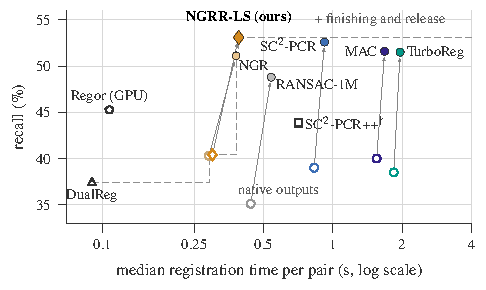
\includegraphics[width=\columnwidth]{figures/fig_pareto.pdf}
\caption{Recall on all 1781 3DLoMatch+FPFH pairs against the median registration-stage time on the 100-pair timing subset (16 CPU threads, MAC 12; \cref{tab:main}). Hollow: native output. Filled: the same frontend with the common finishing and release. Square, triangle, pentagon: native SC$^2$-PCR++, DualReg, Regor (GPU) on the same inputs. $^\dagger$: GPU recall with separate CPU timing. Dashed: CPU Pareto front, excluding $^\dagger$ and Regor. NGRR-LS with the backend has the highest recall; every faster baseline reaches at most 45.3\%.}
\label{fig:pareto}
\end{figure}

\subsection{From candidate coverage to final registration}
\label{sec:verification}
\begin{table}[t]
\caption{Own-process controls. (a) Nested volume inputs, $K=256$, fixed count readout. (b) Same budget/backend; modes: mean distinct poses among 1024; coverage and registrations: pair counts. (c) Cells are frontend--input evaluations. Same ICP and release; Matched K matches finishing calls per cell, Full K uses the top-32 bank. Total calls: 1\,028\,539 for matched/finishing, 1\,474\,185 for full. MAC is excluded from (c).}
\label{tab:units}\centering\footnotesize\setlength{\tabcolsep}{2pt}
\begin{tabular*}{\columnwidth}{@{\extracolsep{\fill}}lrrrr@{}}
\toprule
\multicolumn{5}{@{}l@{}}{\textbf{(a) Dilution: 10 inliers, successes / 40}} \\
Initialization / stages & $N=1000$ & 2000 & 3000 & 4000 \\
\midrule
Uniform / 10 & 11 & 1 & 2 & 0 \\
Pair / 0 & 38 & 11 & 3 & 2 \\
Pair / 10 & 40 & 35 & 29 & 19 \\
Triple / 0 & 36 & 36 & 33 & 26 \\
Triple / 10 & 39 & 37 & 36 & 30 \\
\midrule
\end{tabular*}\par\noindent
\begin{tabular*}{\columnwidth}{@{\extracolsep{\fill}}lrrrr@{}}
\multicolumn{5}{@{}l@{}}{\textbf{(b) Capacity: 3000 training pairs}} \\
Rule & Modes & Raw cover. & Refined cover. & Registered \\
\midrule
Ranking & 222.6 & 2528 & 2429 & 2298 \\
Soft capacity & \textbf{409.6} & \textbf{2639} & \textbf{2487} & \textbf{2326} \\
MMR & 337.8 & \underline{2624} & \textbf{2487} & \textbf{2326} \\
Hard capacity & \underline{363.2} & 2615 & \underline{2467} & \underline{2312} \\
Pose NMS & 243.0 & 2547 & 2438 & 2310 \\
\midrule
\end{tabular*}\par\noindent
\begin{tabular*}{\columnwidth}{@{\extracolsep{\fill}}lrrrr@{}}
\multicolumn{5}{@{}l@{}}{\textbf{(c) Allocation: correct outputs}} \\
Frontend & Cells & Matched K & Full K & Finishing \\
\midrule
RANSAC-1M & 12035 & 9701 & 9729 & \textbf{9771} \\
SC$^2$-PCR & 12035 & 9885 & 9902 & \textbf{9948} \\
TurboReg & 12035 & 9746 & 9783 & \textbf{9886} \\
LGR & 3404 & 2987 & \textbf{2990} & \textbf{2990} \\
NGR & 12035 & 9753 & 9786 & \textbf{9857} \\
\ls{} & 12035 & 9828 & 9843 & \textbf{9920} \\
\midrule
All & 63579 & 51900 & 52033 & \textbf{52372} \\
\bottomrule\end{tabular*}

\end{table}
\begin{table}[t]
\caption{Registration recall (\%) as reported in each paper, next to ours on our inputs (Supp.~Sec.~\ref*{S-sec:s-literature}). *: from another paper's table; $^\dagger$: preprint. Bold / underline: best / second best.}
\label{tab:literature}
\centering\fontsize{7.5}{8.4}\selectfont\setlength{\tabcolsep}{1.5pt}
\begin{tabular*}{\columnwidth}{@{\extracolsep{\fill}}lrrrrrr@{}}
\toprule
 & \multicolumn{2}{c}{3DMatch $\uparrow$} & \multicolumn{2}{c}{3DLoMatch $\uparrow$} & \multicolumn{2}{c}{KITTI $\uparrow$} \\
\cmidrule(lr){2-3}\cmidrule(lr){4-5}\cmidrule(lr){6-7}
Method & FPFH & FCGF & FPFH & FCGF & FPFH & FCGF \\
\midrule
\multicolumn{7}{@{}l@{}}{\emph{Training-free, correspondences only}} \\
TEASER++~\cite{yang2021teaser} & 75.48* & 85.77* & 35.15* & 46.76* & 91.17* & 94.96* \\
SC$^2$-PCR~\cite{chen2022sc2} & 83.98 & 93.28 & 38.57* & 57.83 & \underline{99.64} & 98.20 \\
MAC~\cite{zhang2023mac} & 84.10 & 93.72 & 40.88 & 59.85 & 99.46 & 97.84 \\
FastMAC~\cite{zhang2024fastmac} & 82.87 & 92.67 & 38.46 & 58.23 & 97.84 & 97.84 \\
TurboReg~\cite{yan2025turboreg} & 84.10 & 93.59 & 40.99 & 59.74 & 98.56 & 98.38 \\
FlashReg$^\dagger$~\cite{yu2026flashreg} & 84.01 & 93.41 & 39.25 & 59.12 & 97.83 & 97.66 \\
\multicolumn{7}{@{}l@{}}{\emph{Training-free, using the point clouds}} \\
SC$^2$-PCR++~\cite{chen2023sc2pp} & 87.18 & 94.15 & 41.27* & 61.15 & \underline{99.64} & 98.56 \\
Regor~\cite{zhao2025regor} & 88.48 & 93.96 & 43.96 & -- & \textbf{99.82} & -- \\
DualReg~\cite{li2026dualreg} & 84.41 & 93.65 & 41.66 & 60.86 & 98.20 & 96.58 \\
SVC~\cite{zhang2024svc} & 88.66 & 94.58 & 45.76 & 67.77 & \underline{99.64} & 98.74 \\
\multicolumn{7}{@{}l@{}}{\emph{Learned}} \\
PointDSC~\cite{bai2021pointdsc} & 78.50 & 93.28 & 20.38* & 56.20* & 98.20 & 98.20 \\
VBReg~\cite{jiang2023vbreg} & 82.75 & 93.53 & 32.57* & 58.30 & 98.92 & 98.02 \\
Hunter~\cite{yao2023hunter} & 84.70* & 94.05* & 36.90* & 60.02* & \textbf{99.82*} & -- \\
HyperGCT~\cite{zhang2025hypergct} & 85.89 & 94.45 & 42.28 & 63.73 & 99.10 & 98.92 \\
Decision PCR$^\dagger$~\cite{zhang2025decisionpcr} & 88.29 & \underline{95.13} & 45.54 & \textbf{71.59} & -- & -- \\
\multicolumn{7}{@{}l@{}}{\emph{Ours, on our inputs (training-free unless marked)}} \\
\ls{} (native) & 83.43 & 93.16 & 40.43 & 59.24 & \underline{99.64} & 95.32 \\
SC$^2$-PCR + F+R & \underline{91.00} & 94.89 & 52.55 & 66.98 & \textbf{99.82} & \underline{99.28} \\
\textbf{\ls{} + F+R} & 90.51 & 94.89 & \underline{53.12} & 66.70 & \textbf{99.82} & \textbf{99.46} \\
\ls{} + learned release & \textbf{92.48} & \textbf{95.44} & \textbf{56.20} & \underline{69.12} & \textbf{99.82} & \textbf{99.46} \\
\bottomrule
\end{tabular*}

\end{table}



\Cref{tab:joint} separates the stage gains from candidate coverage and final conversion; \cref{tab:units} tests seeding, retained growth, capacity and allocation. On 3DLoMatch+FPFH, refining only the native NGRR-LS winner reaches 43.0\%. Finishing a selected multi-candidate pool reaches 49.6\%, and release reaches 53.1\% on the same refined pool. For each of the other five frontends, refining the top 32 hypotheses with the same ICP and selecting by truncated correspondence support gives 32 to 72 fewer successes than finishing. Selecting by highest ICP fitness gives 25.3 to 38.4\% recall. On the fixed refined pools of all 63\,579 cells except MAC's, release selects 52\,372 correct cells and exceeds all eight published training-free verification rules we implemented, the best being CorAl~\cite{adolfsson2021coral} (51\,432) and the prerejective score~\cite{buch2013prerejective} (51\,376). On the 39\,590 descriptor-available cells, FS-TCD~\cite{chen2023sc2pp} selects 29\,891 versus 31\,064 for release. Complete rule and per-cohort comparisons are in Supp.~Sec.~\ref*{S-sec:s-selectors}.

\Cref{tab:units}c controls for the actual ICP budget and final decision: matched Top-K uses exactly as many calls as finishing on each cell, with the same SurfaceICP and release. Finishing gains $+693/{-}221$ correct cells; all five correspondence frontends remain significant after Holm correction ($p\le9\times10^{-7}$). On LoMatch+FPFH with NGRR-LS it registers 946/1781 pairs (53.12\%), versus 907/1781 (50.93\%) for matched Top-K. Full Top-32 uses 43.3\% more calls yet registers fewer cells (Supp.~Sec.~\ref*{S-sec:s-topk}).

Capacity raises refined-pool coverage from 56.4\% to 59.2\% on 3DLoMatch+FPFH, while native recall changes only from 40.3\% to 40.4\%. With the same verification, NGR without capacity reaches 51.1\%, compared with 53.1\% for NGRR-LS. The final 946 successes correspond to 89.8\% of the 1054 covered pairs. On FCGF, capacity raises coverage from 70.1\% to 72.0\%, and the complete pipeline selects a correct pose for 92.7\% of covered pairs. Capacity primarily increases the chance that a correct candidate remains available for refinement, while finishing and release convert the resulting pool into registrations.

On fixed NGRR-LS refined pools over nine cohorts, support alone and shape alone yield 9760 and 9759 successes, while their minimum yields 9920. Product and harmonic mean perform similarly across frontends. A weighted sum fitted on training data improves NGRR-LS to 9992, and an optional learned release reaches 10\,084. The shape null is not calibrated on real wrong poses, but the score ranks candidates with AUC 0.83 to 0.99 (\supp{\cref*{S-sec:s-verification,S-tab:s-rules}}). The stage diagnostics divide NGRR-LS's 835 failed 3DLoMatch+FPFH outputs into 727 pairs without a correct refined candidate and 108 pairs with one that release does not select. The latter group isolates errors in final selection within an existing candidate pool.

\subsection{Nucleus crowding and capacity control}
\label{sec:crowding}

NGR's first 256 candidates contain 69.5 distinct poses, versus 164.7 to 214.6 for the baselines (\supp{\cref*{S-fig:s-crowding}}a). Capacity raises rank-1024 coverage from 2528 to 2639 pairs and the refined-pool ceiling from 2429 to 2487 (+71/$-$13), at 1.13$\times$ the time. Doubling nuclei adds 18 covered pairs at 1.64$\times$ (\supp{\cref*{S-fig:s-crowding}}c). Across nine cohorts, capacity adds 134 covered pairs and 63 training-free registrations.

The same-budget comparison in \cref{tab:units}b isolates the capacity rule; full diversity and timing measures are in Supp.~Tab.~\ref*{S-tab:s-diversity}. Soft capacity and MMR tie on refined coverage and final registrations, both exceeding hard capacity and pose suppression. This supports soft penalties on repeated use of matches. In a decoy test with ten true matches and a 40-match false rigid cluster, capacity raises correct-pose coverage from 0/100 to 100/100. Consensus-only selection still chooses the wrong motion.

\subsection{Stress tests and extreme sparsity}
\label{sec:synthetic}
\begin{figure}[t]
\centering
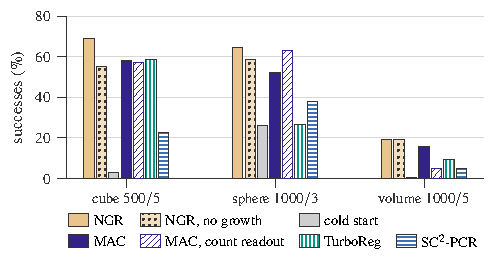
\includegraphics[width=\columnwidth]{figures/fig_sparse.pdf}
\caption{Frozen synthetic benchmark (250 inputs per setting, $N/m$: matches/inliers). Inliers are noisy transformed points, and outliers are uniform in the unit cube (cube), in a radius-5 ball (sphere) or in the object's bounding box (volume). Success: RE $<5^\circ$, TE $<0.05$. The same NGR seeds are fitted directly or grown. MAC is the authors' C++ code with its compatibility width fixed to 0.75$\tau$ (\supp{\cref*{S-sec:s-maccpp}}); hatched bars show it with NGR's count readout. On the volume background, NGR uses MAE and MAC keeps its own choice. Full protocols and fresh draws are in Supp.~Sec.~\ref*{S-sec:s-synthetic}.}
\label{fig:sparse}
\end{figure}

\Cref{tab:units}a isolates seeded growth on the dilute volume inputs: pair nuclei improve from 2/40 without growth to 19/40 with ten stages. Resetting half the composition each stage removes most of the pair-seeded gain, supporting retained enrichment.

On the frozen cube setting in \cref{fig:sparse}, removing growth lowers NGR from 69.2\% to 55.2\%. With three sphere-background inliers among 4000 matches, NGR registers 29/100 inputs versus at most 4/100 for SC$^2$-PCR and TurboReg. On real scans thinned to 5 to 20 inliers no frontend consistently leads. Full grids and tests are reported in \supp{\cref*{S-sec:s-synthetic}}.

\subsection{Generalization and efficiency}
\label{sec:cost}
Verification improves every tested frontend on ETH, which was not used for algorithm-adoption decisions. NGRR-LS rises from 78.1\% to 98.7\%. Under GeoTransformer's official scene-mean criterion, verification improves every frontend by 0.5 to 2.4 percentage points on 3DLoMatch and 0.4 to 1.0 on 3DMatch. LGR rises from 74.03\% to 75.77\% on 3DLoMatch. NGRR-LS does not rank first on these learned correspondences (\supp{\cref*{S-tab:s-official}}).

Published results obtained with different inputs or processing are reported separately in \cref{tab:literature}.

\paragraph{Measured cost of conversion.}
The compiled frontend restricts phase growth to initial supports with non-negligible weight and avoids negligible triplet terms. Dense products are retained when supports are large. Finishing compiles ICP and suppression, uses exact thresholded surface queries on a spatial grid, and computes release moments in place. These CPU changes reduce the timed NGRR-LS stages to 0.78\,s at four threads and 0.39\,s at sixteen on the timed cohort. The 16-thread result appears in \cref{tab:main}, and the four-thread result appears in \supp{\cref*{S-tab:s-cost}}.

The final implementation preserves the success/failure indicators for native output, refined-pool coverage and final release on all 15\,035 checked train/test inputs. Frontend speedups range from 3.3 to 7.2$\times$ on FPFH cohorts to 1.4 to 4.4$\times$ on learned correspondences. Switches were calibrated for runtime on separate inputs. Validation details are in \supp{\cref*{S-sec:s-cost}}.


\section{Discussion and conclusion}
\label{sec:conclusion}

We present a chemical-process-inspired framework that organizes robust registration as the recovery, preservation, enrichment, refinement and selection of pose hypotheses. Motif nucleation introduces geometrically supported candidate phases, site capacity discourages repeated clusters of matches from consuming the nucleus budget, and retained growth enriches each phase from its current composition.

Finishing allocates a fixed refinement budget across diverse pose hypotheses and refines them on the observed surfaces. Release then selects from the refined pool using complementary support and residual-shape evidence. The shared-ICP controls isolate the contributions of candidate allocation and final selection.

Capacity raises refined-pool coverage on 3DLoMatch+FPFH from 56.4\% to 59.2\%, although its native recall changes from 40.3\% to 40.4\%. Finishing and release raise NGRR-LS from 43.0\% with winner-only ICP to 49.6\% and 53.1\%. The complete pipeline selects a correct pose for 89.8\% of covered pairs. Applying the same verification procedure to six different frontends raises recall by 10.8 to 13.7 percentage points on 3DLoMatch+FPFH.

In the controlled dilution experiments, seeded growth improves recovery when a small correct set must be enriched. On real pairs with very few inliers, candidate coverage and final selection both remain difficult. The diversity and score controls further delimit the roles of site capacity and release (\supp{\cref*{S-sec:s-limitations}}).

The gains across heterogeneous frontends suggest that a frontend's final estimate does not fully characterize its registration potential. The gap between native recall and refined-pool coverage supports this interpretation. We therefore view registration as a budgeted process of recovery and conversion. Under a fixed refinement procedure, candidate coverage and conditional selection effectiveness should be measured separately.

\label{page:bodyend}
\section*{LLM Usage Statement}
The authors independently proposed the core research ideas and the chemical-process formulation. The authors used Anthropic's Claude (through Claude Code) and OpenAI's ChatGPT/Codex for literature research, language polishing, assistance with code writing, and organization of experimental results. The authors take responsibility for the methods, implementation, citations and reported results.

\clearpage
\label{page:backmatter}

{
    \small
    \bibliographystyle{ieeenat_fullname}
    \bibliography{references}
}


\clearpage
\setcounter{section}{0}
\setcounter{figure}{0}
\setcounter{table}{0}
\setcounter{equation}{0}
\renewcommand{\thesection}{S\arabic{section}}
\renewcommand{\thefigure}{S\arabic{figure}}
\renewcommand{\thetable}{S\arabic{table}}
\renewcommand{\theequation}{S\arabic{equation}}
\renewcommand{\theHsection}{S\arabic{section}}
\renewcommand{\theHfigure}{S\arabic{figure}}
\renewcommand{\theHtable}{S\arabic{table}}
\renewcommand{\theHequation}{S\arabic{equation}}
\maketitlesupplementary
\section{Chemical operations and the registration pipeline}
\label{S-sec:s-flowsheet}

Chemical separation uses different operations to recover a product and assess its quality~\cite{mccabe2005,mullin2001}. Seed crystals initiate a product phase in a dilute solution. Finite adsorption capacity limits how much a species can occupy a site. A column under total reflux returns enriched condensate and retains its composition between stages. Finishing improves the recovered products before a release assay checks their specifications. In registration, the corresponding tasks are to generate a correct hypothesis and to select it from the candidates.

The registration pipeline follows these operations (\main{\cref*{fig:flowsheet}}). Its generation section was designed from the first three units: geometric motifs seed the candidate phases, a finite site capacity keeps any single cluster of wrong matches from taking every seed, and total-reflux growth enriches each phase from its own composition. Multi-stream finishing refines candidates on the observed surfaces. A release test then selects a pose by its limiting specification. These verification stages can follow any frontend. We test each operation by removing or replacing it (\cref{S-tab:s-process}; \main{\cref*{tab:units}} summarizes seed/growth and capacity controls). The mapping specifies computational operations; it does not model crystallization or adsorption equilibria.

\paragraph{Reading the flowsheet figure.} \main{\cref*{fig:flowsheet}} shows the chemical flowsheet above the algorithm's data-flow network, with matching stream numbers for corresponding connections. The input is a 3DLoMatch+FPFH pair with 2.9\% inliers (green; outliers red). The native \ls{} output misses this pair (TE 36\,cm), while the full pipeline registers it (RE 4.1$^\circ$, TE 19\,cm). The heatmaps represent compatibility and motif scores. Ranking by compatibility alone concentrates triple nuclei in one cluster; the Langmuir vacancy $\theta_x=1/(1+n_x/q)$ spreads the budget over clusters. Each nucleus grows over compatible matches for ten stages that retain the current composition, then yields a rigid hypothesis. Point-to-plane ICP refines up to 32 hypotheses on the observed surfaces. Release ranks each candidate by the weaker of its normalized support $s$ and residual-shape $h$ specifications. Generation is blue and verification is amber. The verification stages also accept other frontends' hypotheses. The arrow strip reports recall on 3DLoMatch+FPFH (1781 pairs) with \ls{}: 40.4\% after generation, 49.6\% after finishing and 53.1\% after release. The refined-pool ceiling is 59.2\%. Diamonds 1--7 identify corresponding connections, including 3 for growth stages and total reflux and 7 for scans and the sample line. The heatmaps, bars and equipment are schematic.

\begin{table*}[t]
\caption{Unit operations, their computational roles and the interventions used to test them. \main{\cref*{tab:units}} gives compact seed/growth and capacity controls. The first three rows concern the \ngr{} frontend; finishing and the release assay apply to every frontend. Synthetic numbers are successes out of 40 inputs with $m=10$ inliers among $N=4000$ matches on the volume background, from the original estimator configuration with $K=256$ nuclei (\cref{S-sec:s-synthetic}). Training numbers use the 3000 FPFH pairs of the 3DMatch training cohort; time factors are mean frozen frontend times relative to \ngr{}. The remaining real-data results use the test cohorts of \main{\cref*{sec:experiments}}. Section numbers in the second column refer to the main paper.}
\label{S-tab:s-process}
\centering\small
\renewcommand{\arraystretch}{1.12}
\begin{tabularx}{\linewidth}{@{}>{\raggedright\arraybackslash}p{2.55cm}>{\raggedright\arraybackslash}p{4.1cm}X@{}}
\toprule
Unit operation & Registration step & Intervention and measured effect \\
\midrule
Seeded nucleation & Pair and triple motifs of the compatibility graph seed $K$ independent phases (\cref*{sec:nucleation}) & Seeds replaced by a uniform start (cold start): synthetic successes 19/40 (pairs) and 30/40 (triples) fall to 0/40 \\
Finite site capacity (Langmuir) & A nucleus's affinity is multiplied by the vacancies $\theta_x=1/(1+n_x/q)$ of its matches (\cref*{sec:capacity}) & Removed (\ngr): training pairs with a correct refined candidate 2487 $\to$ 2429; twice the nuclei instead: 2447 at 1.64$\times$ the frontend time (site capacity: 1.13$\times$) \\
Total reflux & Ten multiplicative growth stages retain the current composition (\cref*{sec:reflux}) & Growth removed: 19/40 $\to$ 2/40 with pair nuclei, 30/40 $\to$ 26/40 with triples; pair-seeded composition reset to the nucleus at every stage: 19/40 $\to$ 4/40 \\
Multi-stream finishing & Up to 32 candidates refined by two-scale ICP on the observed surfaces (\cref*{sec:finishing}) & Replaced by ICP of the native winner: 3DLoMatch+FPFH recall 49.6\% $\to$ 43.0\% (\ls); by top-32 + the same ICP + selection by correspondence support: 32--72 fewer pairs for each of RANSAC, SC$^2$-PCR, MAC, TurboReg and \ngr{} \\
Release assay & The candidate whose weaker normalized specification, support ($M\sqrt{I}$) or residual shape, is best (\cref*{sec:assay}) & Replaced by the finishing step's anchor rule: 133--189 fewer pairs for each of the five frontends run on all nine cohorts; 3DLoMatch+FPFH 53.1\% $\to$ 49.6\% (\ls) \\
\bottomrule
\end{tabularx}

\end{table*}

\paragraph{Process analogies in computation.} Simulated annealing~\cite{kirkpatrick1983annealing} applies a rule from materials processing to optimization. Here the analogies specify unit operations whose computational roles can be tested by intervention.
\FloatBarrier
\section{Method details}
\label{S-sec:s-method}

The method in \main{\cref*{sec:method}} takes $N$ putative matches $(p_i,q_i)\in\mathbb{R}^3\times\mathbb{R}^3$ and two observed point clouds as input, and returns a rigid motion $(R,t)$. The \ngr{} frontend generates pose hypotheses from the matches. Verification refines several candidates and selects one pose; it can accept hypotheses from any frontend.

\paragraph{Seeded nucleation.} The seeds are geometric motifs of the zero-diagonal compatibility graph $\Lambda$ of \main{\cref*{eq:compat}}. The kernel width is $\sigma_c=0.375\tau$ (3.75\,cm indoors). Pairs are ranked by the second-order compatibility $\Lambda_{ab}(\Lambda^2)_{ab}$ of SC$^2$-PCR~\cite{chen2022sc2} and triples by $T_{abc}=\Lambda_{ab}\Lambda_{bc}\Lambda_{ca}\sum_d\Lambda_{ad}\Lambda_{bd}\Lambda_{cd}$, with a non-degeneracy test on both triangles, $(p_a,p_b,p_c)$ and $(q_a,q_b,q_c)$. Each selected motif seeds one phase, a probability vector over all matches: $w_i^{(0)}\propto\Lambda_{ai}\Lambda_{bi}+\delta_{ia}+\delta_{ib}$ for a pair $(a,b)$ and $w_i^{(0)}\propto\Lambda_{ai}\Lambda_{bi}\Lambda_{ci}+\delta_{ia}+\delta_{ib}+\delta_{ic}$ for a triple $(a,b,c)$. Every match therefore starts with positive weight. A background-load scheduler computes $(N-2)\bar\Lambda^2$, the number of supporting triangles a pair expects from the background ($\bar\Lambda$ is the mean off-diagonal compatibility). Below one it uses 256 pair seeds and the count readout. Otherwise a shortlist of 4096 pairs is extended to $K=1024$ triples with the MAE readout. All $K$ phases evolve independently.

\paragraph{Candidate crowding.} Ranking motifs by compatibility alone allows a single cluster to occupy the entire seed budget. A cluster of $n$ mutually compatible wrong matches has $\binom{n}{2}$ internal pairs, each supported by about $n-2$ triangles (4095 pairs with support near 89 for $n=91$), whereas among $m$ true inliers a true pair collects about $m-2$, only 8--23 for the 10--25 inliers typical of hard pairs. A few such clusters can then take most of the pair shortlist and the nuclei, and the pool concentrates on a few poses (\main{\cref*{sec:crowding}}; \cref{S-sec:s-crowding}).

\paragraph{Finite site capacity.} In competitive adsorption a surface site holds a limited amount of adsorbate, so a dominant species saturates its own sites and leaves the rest for others~\cite{langmuir1918}. Every match $x$ carries the site vacancy $\theta_x=1/(1+n_x/q)$ of \main{\cref*{eq:vacancy}}, where $n_x$ counts the already selected motifs that contain $x$. We discount a candidate motif's affinity by the vacancies of its matches, $T_{abc}\,\theta_a\theta_b\theta_c$ (pairs analogously). The first half of the pair shortlist and of the nuclei keep the original ranking. The second half is filled greedily by discounted affinity from a deeper ranking (65\,536 pairs, 16\,384 triples), counting every selected motif as occupying its sites. The capacities $q=8$ for pairs and $q=4$ for triples were fixed when the variant was pre-registered and never tuned (\cref{S-sec:s-protocol}). Growth, fitting and scoring are unchanged; the resulting frontend is \ls{}. The vacancy is an occupancy feedback in Langmuir form, not a derived adsorption equilibrium.

\paragraph{Relation to diversity selection.} The vacancy penalizes a motif according to how often its matches have already been selected. The penalty is cumulative and soft. Other diversity rules act differently on the same ranked list. Maximal marginal relevance~\cite{carbonell1998mmr} on the match sets, with its default trade-off $\lambda=\frac12$, subtracts the largest overlap with any single selected motif. A hard capacity rejects a motif once one of its matches is held $q$ times (a match may sit in at most 8 pairs or 4 triples); when no admissible motif is left, the remaining nuclei are taken in ranking order. Non-maximum suppression in pose space rejects a nucleus whose three-point pose repeats an earlier one. \main{\cref*{sec:crowding}} and \cref{S-tab:s-diversity} compare the four rules with the same budget, first halves and deep rankings. The two soft rules on match reuse tie; both reach a higher ceiling than hard capacity and pose suppression.

\paragraph{Total-reflux growth, refits and pool score.} Each phase is grown for ten stages by \main{\cref*{eq:growth}} with $\epsilon=1$ and $\beta=2$. The factor $w_i^{(s)}$ multiplies the support by the current composition and retains the enrichment from the previous stage. All matches stay available; only the number of phases is capped. Each grown phase gives a weighted Kabsch fit~\cite{kabsch1976}, followed by two hard refits with residual radius $\tau_c=\tau$ (0.04 in the frontend's internal units, where $\tau$ maps to 0.04). The triple branch scores the pool by $\sum_i[1-r_i/\tau_c]_+$ on the matches, where $r_i$ is the residual of match $i$ under the hypothesis.

\paragraph{Multi-stream finishing.} Finishing keeps the frontend's native winner, shortlists geometrically distinct candidates ($5^\circ$ and $\tau$ pose suppression), and fills at most $B=32$ refinements: up to 16 primary modes allocated by interleaved rankings of three supports, then extra modes from the non-dominated set. Each selected candidate is refined by point-to-plane ICP~\cite{besl1992icp,chen1992medioni} on the observed surfaces at radii $2\tau$ and $\tau$ ($\tau=0.1$\,m indoors, 0.3\,m on ETH, 0.6\,m on KITTI). For each refined pose $h$ it records the truncated correspondence support $M(h)$, the bidirectional surface support $G(h)$, and an information-weighted support $I(h)$ whose query weights are the leverages $\ell_i=J_i(\sum_jJ_j^\top J_j)^{\dagger}J_i^\top$ of the point-to-plane rows $J_i=[(\widetilde x_i\times n_i)^\top,n_i^\top]$~\cite{gelfand2003stable}, with $\widetilde x_i$ the centered and scale-normalized query point and $n_i$ its normal. The weights are computed once on each cloud's query points and do not depend on the pose. The finishing-only output keeps the candidate with the largest $M\sqrt{G}$ as an anchor. A challenger replaces it only if it raises $M\sqrt{I}$ without lowering $I$. This anchor rule is the baseline over which the release assay had to pass its pre-registered margin (\cref{S-sec:s-protocol}). The same finishing procedure runs after every frontend, without labels or learned weights.

\paragraph{Release assay: two specifications.} The assay checks two specifications of each refined candidate $k$ in the refined pool $V$. The \emph{support} channel measures how much of the scene the pose explains, $s_k=M_k\sqrt{I_k}/\max_{j\in V}M_j\sqrt{I_j}$. The \emph{shape} channel measures how tightly the supported points lie on the other surface. For the $m$ query points whose nearest-neighbor distance $d$ is below $\tau$, let $u=d^2/\tau^2$ and $\bar u=\frac1m\sum u$.

\paragraph{The null and the Cram\'er rate.} We choose the idealized radial reference $p_0(d)=2d/\tau^2$ on $[0,\tau)$, motivated by uniform area in a planar disc. It gives $\Pr(d\le r\mid d<\tau)=r^2/\tau^2$. Hence $u$ is uniform on $[0,1)$, $\bar u\approx\frac12$, and $\mathbb{E}\,e^{-\beta u}=(1-e^{-\beta})/\beta$. The Cram\'er rate of a smaller mean under this null is the Legendre transform of $\log\mathbb{E}\,e^{-\beta u}$,
\begin{equation}
\psi(\bar u)=\sup_{\beta\ge0}\Big\{-\beta\bar u-\log\frac{1-e^{-\beta}}{\beta}\Big\},
\label{S-eq:s-psi}
\end{equation}
which is \main{\cref*{eq:psi}}. If the $m$ null residuals are independent, the probability that their mean is at most $\bar u<\frac12$ is bounded by $e^{-m\psi(\bar u)}$ (Chernoff's bound). As $m$ grows, this probability decays at that rate (Cram\'er's theorem), so $\psi$ measures per-point evidence of residual concentration. The objective in braces is concave in $\beta$, vanishes at $\beta=0$ and has slope $\frac12-\bar u$ there, so $\psi$ is zero for $\bar u\ge\frac12$ and positive below. Averaging $\psi$ over the two directions (source queries against the target surface and target queries against the source surface) gives $J_k$, and $h_k=\exp(J_k-\max_{j\in V}J_j)$. The assay releases $\hat k=\arg\max_{k\in V}\min\{s_k,h_k\}$ (\main{\cref*{eq:assay}}), breaking ties by $s_k$, then $h_k$, then queue order. The definitions fix the constants without fitting.

\paragraph{Minimax-regret interpretation.} Consider the surrogate utility $U_\lambda(k)=\lambda s_k+(1-\lambda)h_k$ of candidate $k$ for an unknown exchange rate $\lambda\in[0,1]$. The regret of choosing $k$ is
\begin{equation}
r_k(\lambda)=\max_{j\in V}U_\lambda(j)-U_\lambda(k).
\label{S-eq:s-regret}
\end{equation}
Its first term is a maximum of functions affine in $\lambda$ and therefore convex, and its second term is affine, so $r_k$ is convex on $[0,1]$ and attains its maximum at an endpoint. Both channels are normalized to a maximum of one over $V$ ($\max_j s_j=1$ by definition and $\max_j h_j=e^0=1$), so $r_k(0)=1-h_k$ and $r_k(1)=1-s_k$. The worst-case regret is the larger of the two, $\max\{1-s_k,1-h_k\}$:
\begin{equation}
\max_{\lambda\in[0,1]}r_k(\lambda)=1-\min\{s_k,h_k\}.
\label{S-eq:s-worst}
\end{equation}
Minimizing the worst-case regret over $k\in V$ is therefore exactly the release rule of \main{\cref*{eq:assay}}. The guarantee concerns this family of surrogate utilities, not registration success itself, and the null behind $\psi$ is an idealization. On real scans, the null is not calibrated, although $\psi$ helps rank candidates. The product and harmonic mean of the two channels perform similarly to the release rule. A weighted sum with one weight fitted on the training cohort succeeds on about 0.5\% more frontend-pair evaluations (\main{\cref*{sec:verification}}; \cref{S-sec:s-verification}).

\paragraph{Optional learned assay.} The learned assay is a conditional logit over the candidates of a pool (a softmax over the pool of a linear score of each candidate's features) with 26 label-free features of the finishing quantities, trained only on the 3DMatch training scenes. We chose its features, regularization and weights on the training cohort. The candidate features had been listed before the protocol was in place (\cref{S-sec:s-protocol}). We report this variant separately from all training-free results.
\FloatBarrier
\section{Evaluation protocol}
\label{S-sec:s-protocol}

The protocol summarized in \main{\cref*{sec:protocol}} distinguishes pre-registered decisions from earlier development.

\paragraph{Cohorts.} We use the nine test cohorts in \main{\cref*{sec:experiments}} (12\,035 pairs): 3DMatch and 3DLoMatch with FPFH, FCGF and GeoTransformer correspondences, KITTI with FPFH and FCGF, and ETH with FPFH, an outdoor laser dataset used neither for training nor for any adoption decision. The training cohort is 3000 FPFH pairs from 82 3DMatch training scenes, disjoint from every test scene.

\paragraph{Predating the protocol.} The \ngr{} frontend and finishing procedure were fixed before this protocol. Their development included public-benchmark evaluations, so those benchmarks were not held out for these components.

\paragraph{Under the protocol.} The two components added here, the finite site capacity and the release assay of \main{\cref*{eq:assay}}, were each pre-registered in writing before their first run. The registration specified the rule, constants, adoption margin and, for the assay, a predicted range. Adoption decisions used only the training cohort. \ls{} was the only one of four pre-registered frontend variants to pass its margin; two larger-budget controls, the doubled and tripled nuclei, were pre-registered alongside. The assay passed its margin over the finishing step's own rule, the anchor rule of \cref{S-sec:s-method}. Each adopted component was then run once on the test cohorts. A further pre-registered component filled unused ICP slots with more candidates. It passed the training-cohort margin by raising the refined-pool ceiling (+37 pairs) while leaving the finishing step's own choice essentially unchanged there (2242 against 2243 registered pairs). Its single test run raised the ceiling by 58 of 12\,035 pairs and the released count by 2, so the reported pipeline does not use it (see below and \cref{S-tab:s-fill}). No other test result under this protocol informed a design choice.

\paragraph{Partly under the protocol.} The optional learned assay chose its features, regularization and weights on the training cohort only, but its 26 candidate features were listed before the protocol was in place: 13 come from an earlier learned readout that had been evaluated on test data, and 13 were added after that evaluation. We report the learned assay separately from the training-free results.

\paragraph{Comparisons added later.} The comparison of the site capacity with other diversity rules (\main{\cref*{sec:crowding}}; \cref{S-sec:s-crowding}) and that of the release rule with other combinations of its two channels (\main{\cref*{sec:verification}}; \cref{S-sec:s-verification}) were added after the main evaluation; each was pre-registered before it was run, and neither changes the reported pipeline.

\paragraph{Statistics and conventions.} Paired differences use McNemar's test~\cite{mcnemar1947}; tests over several cells, such as the conditions of a synthetic grid or the rules of one comparison, use Holm's correction. A paired count $+a/{-}b$ gives the pairs (or cells) registered by the first method and not by the second ($a$), and the reverse ($b$). In the comparison of release rules a cell is one pair with the refined pool of one frontend; the cells of one pair share its scans and correspondences, so $p$ is from a sign test over pairs. Refined-pool coverage, also called the ceiling, counts pairs with at least one correct refined pose. It depends on generation and finishing and bounds release on a fixed pool. 3DLoMatch contains only eight test scenes, so absolute recall has substantial scene-level uncertainty; \main{\cref*{sec:product}} gives scene-bootstrap intervals for the paired gains, and \cref{S-sec:s-results} also for recall.

\paragraph{Filling the unused ICP slots.} With \ls{}, the finishing step uses on average 12.6 of its 32 ICP slots over the nine test cohorts. A pre-registered extension fills unused slots from the remaining shortlist, then from further non-dominated layers. It retains every original refinement, so coverage cannot decrease. On the training cohort it raised the ceiling from 2487 to 2524 pairs ($+37/{-}0$), passing its pre-registered margin, and left the finishing step's own choice essentially unchanged (2242 against 2243 registered pairs). \Cref{S-tab:s-fill} gives its single run on the nine test cohorts: the ceiling rises by 31--70 pairs for every frontend, but the released count changes by 0 to 16 pairs. The reported pipeline therefore does not use it.

\begin{table}[t]
\caption{Registered pairs over the nine test cohorts (12\,035 pairs) before and after filling the unused ICP slots, in its single test run. Ceiling: a correct pose among the refined candidates. + finishing: the finishing step's own choice; + release: the release assay; + learned release: the optional learned assay. MAC was not run.}
\label{S-tab:s-fill}
\centering\scriptsize
\setlength{\tabcolsep}{2.5pt}
\begin{tabular}{@{}lrrrr@{}}
\toprule
Frontend & Ceiling & + finishing & + release & \begin{tabular}[b]{@{}r@{}}+ learned\\release\end{tabular} \\
\midrule
\ls{} & $10292{\to}10350$ & $9752{\to}9754$ & $9920{\to}9922$ & $10084{\to}10095$ \\
\ngr{} & $10158{\to}10216$ & $9724{\to}9719$ & $9857{\to}9857$ & $9969{\to}9978$ \\
SC$^2$-PCR & $10377{\to}10447$ & $9759{\to}9763$ & $9948{\to}9953$ & $10117{\to}10135$ \\
TurboReg & $10207{\to}10238$ & $9748{\to}9754$ & $9886{\to}9895$ & $10024{\to}10046$ \\
RANSAC-1M & $10074{\to}10113$ & $9613{\to}9621$ & $9771{\to}9787$ & $9887{\to}9911$ \\
\bottomrule
\end{tabular}

\end{table}
\FloatBarrier
\section{Synthetic studies}
\label{S-sec:s-synthetic}

\paragraph{C++ MAC in the main synthetic figure.}
The main figure uses the completed 750-input C++ experiment from the author's 3DMatch/FPFH branch. Coordinates are scaled by 2.5 to match the release's 0.1 inlier radius to the synthetic $\tau=0.04$; the point-spacing parameter is overridden so the effective compatibility width is $0.75\tau$. All other graph, clique-selection and native-refinement decisions are retained. Each setting has 250 inputs. Native successes are 146/131/39 for cube/sphere/volume; count-readout successes on the same pools are 143/158/13. Native outcomes agree with the stored array implementation on 749/750 inputs; the count-readout outcomes agree on all 750. Fresh grids, decoys and thinned scans below retain their labelled array implementation.

\subsection{The frozen synthetic benchmark}

The benchmark, random seeds and baseline parameters were fixed before this study. We reproduce the inputs from those seeds without changing the protocol. Each of its three conditions has 250 inputs. We identify a condition by its outlier background and $N/m$, the numbers of matches and generated inliers: cube $500/5$, sphere $1000/3$ and volume $1000/5$. The benchmark also specifies three descriptive control conditions (sphere $1000/5$, volume $1000/3$ and cube $1000/5$), which we do not use. All inputs derive from the master seed 2026102801.

\paragraph{Sphere and volume.} The source cloud is the Stanford Bunny~\cite{stanford} (\texttt{bun\_zipper.ply}, 35\,947 vertices), shifted by its coordinatewise minimum and divided by its largest coordinate span to fit within a unit-side bounding box. Each input draws a fresh 4000-vertex source sample of the Bunny, a Haar-distributed rotation and a translation uniform in the unit ball. The $m$ generated inliers are chosen among the first 1000 source vertices; their targets are the transformed source points plus Gaussian noise with coordinate standard deviation 0.01, resampled when its norm exceeds 0.0554. All remaining targets are background points. For the \emph{sphere} condition, each background target is uniform in the origin-centered ball of radius five, the known-scale setting of the TEASER experiments~\cite{yang2021teaser}. For the \emph{volume} condition, each background target is uniform in the axis-aligned bounding box of the normalized Bunny and then moved by the true motion, so the outliers overlap the object.

\paragraph{Cube.} Source points and outlier points are uniform in $[0,1]^3$. The rotation is the QR factor of a Gaussian matrix with sign correction, and the translation has independent Gaussian coordinates with standard deviation 0.5. An inlier's target is $Rp_i+t+\eta_i$ with $\eta_i\sim\mathcal{N}(0,0.01^2I)$; an outlier's target is $Ru_i+t$ for an independent uniform point $u_i$. Cube inputs are generated one at a time from their own trial seeds.

\paragraph{Shared protocol.} The matches are shuffled after the inliers are placed, and every estimator receives the same coordinate arrays. The number $m$ counts generated inliers. Outliers that happen to lie near the true pose remain in the input and are excluded from $m$. All synthetic studies in this section count a registration as successful when the returned pose has rotation error below $5^\circ$ and translation error below 0.05. Evaluation adds no refitting. Baseline parameters were calibrated on separate development inputs before the benchmark was drawn: for MAC graph scale 0.3, cutoff 0.99 and verification radius 0.04; for TurboReg length threshold 0.015 and NMS radius 0.04; for SC$^2$-PCR $d=0.02$, $k_1=10$, $k_2=5$ and radius 0.04. The fresh-draw experiments also use the original baseline parameters: MAC graph scale 0.4, TurboReg length threshold 0.02 and SC$^2$-PCR $d=0.04$.

\paragraph{Readouts.} \ngr{} selects among its refined candidates with one of two extensive scores of the residuals $r_i$, at radius $\tau_c=0.04$. With pair nuclei it uses the \emph{count readout} $\sum_i\mathbf{1}[r_i<\tau_c]-10^{-3}\,\frac1N\sum_i r_i$, a support count with a small residual tie-break; with triple nuclei it uses the \emph{MAE score} $\sum_i[1-r_i/\tau_c]_+$ (\cref{S-sec:s-method}). On this benchmark the background-load scheduler chooses pair nuclei on the cube and sphere backgrounds and triple nuclei on the volume background. ``MAC, count readout'' keeps MAC's graph, candidate pool and winner refinement and replaces only its selection score by the count readout.

\subsection{Seed and reflux interventions}

\begin{figure}[t]
\centering
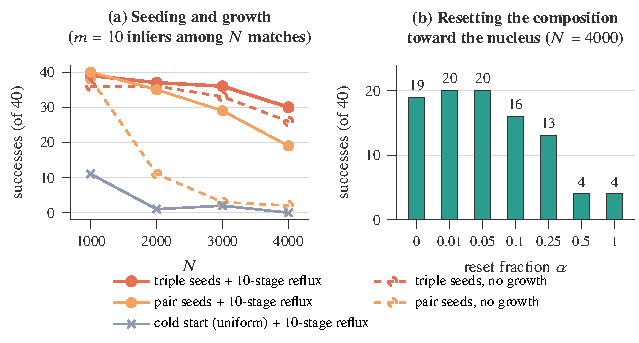
\includegraphics[width=\linewidth]{shared/figures/fig_mechanism.pdf}
\caption{Interventions on the seeding and reflux units (synthetic volume background, $m=10$ generated inliers among $N$ matches, 40 inputs per point; the original estimator configuration with $K=256$ nuclei). (a) Without seeds, growth fails as the feed is diluted; pair seeds without growth fail as well, while purer triple seeds gain less from growth. (b) Resetting a fraction $\alpha$ of each stage's composition to the pair nucleus removes most of the benefit at $\alpha\ge0.5$.}
\label{S-fig:s-mechanism}
\end{figure}

\Cref{S-fig:s-mechanism} removes the seeding and reflux units one at a time on synthetic inputs with ten inliers, using the original estimator configuration ($K=256$ nuclei, the count readout and two hard refits). The inputs use an earlier draw of the Bunny volume generator (master seed 2026102501 and one fixed 4000-vertex source sample). Across the four values of $N$, we retain the same ten inliers, noise, pose and all matches present at smaller $N$. Without seeds, ten stages of growth from a uniform start recover 11/40 inputs at $N=1000$ and 0/40 at $N=4000$. With pair seeds the same growth recovers 40/40 and 19/40, and triple seeds recover 39/40 and 30/40. Without growth, pair-seeded success falls from 38/40 to 2/40 as $N$ grows, while triple seeds start purer and gain less from growth (26/40 to 30/40 at $N=4000$). We test retention by resetting part of each pair-seeded phase toward its initial composition at every stage: the factor $w_i^{(s)}$ of \main{\cref*{eq:growth}} is replaced by $(1-\alpha)w_i^{(s)}+\alpha w_i^{(0)}$. The support factor still uses the current composition. Thus $\alpha=0$ gives the original update, while $\alpha=1$ reapplies the nucleus weights at every stage. Small resets ($\alpha\le0.05$) change little, and $\alpha\ge0.5$ leaves 4/40.

\subsection{Removing units on the frozen benchmark}

The frontend was designed for correspondence sets with very few correct matches. Real benchmarks contain such pairs (\main{\cref*{sec:product}}) but do not allow direct control of the inlier count, which motivates the synthetic tests. We regenerate the benchmark from its fixed seeds and remove one unit at a time (\main{\cref*{fig:sparse}}), and then draw fresh inputs (\cref{S-sec:s-fresh}). The frozen \ngr{} and TurboReg reproduce the recorded counts exactly; the updated C++ MAC differs from the earlier array implementation on one cube input. SC$^2$-PCR, rerun here, registers 57, 95 and 13 of the 250 inputs on the cube, sphere and volume conditions, compared with the recorded counts of 52, 95 and 14. The arms of \main{\cref*{fig:sparse}} are ``no growth'', the same nuclei fitted directly, and ``cold start'', one uniform phase grown for ten stages. Here we also report ``MAC, count readout'': the width-matched C++ MAC candidates selected by the count readout that \ngr{} applies to pair nuclei; on the volume background the native MAC bar retains its own MAE choice, while the count-readout bar is a separate control.

On the cube condition (five inliers among 500 matches) \ngr{} registers 69.2\% of the inputs, against 58.4\% for the width-matched C++ MAC (\cref{S-sec:s-maccpp}) and 58.8\% for TurboReg (paired $+54/-27$ and $+54/-28$, Holm $p<0.01$). On the sphere condition (three inliers among 1000 matches) it registers 64.8\% against 52.4\% for MAC and 26.4\% for TurboReg ($+100/-4$ against TurboReg, Holm $p=10^{-24}$). On the volume condition, it registers 19.2\% against 15.6\% for MAC (not significant) and 9.2\% for TurboReg ($+35/-10$, Holm $p=5\times10^{-4}$). On the cube, fitting the same seeds without growth lowers recall to 55.2\%, below both baselines ($+57/-22$ for growth, Holm $p=3\times10^{-4}$), and a cold start reaches 3.2\%. On the sphere growth adds $+18/-3$ under \ngr{}'s count readout (with the MAE readout both reach 130). The readout accounts for part of this difference: MAC with \ngr{}'s count readout reaches 63.2\%, not significantly below 64.8\%. With triple nuclei (volume background) growth leaves \ngr{}'s output unchanged (48 either way); its pools contain a correct pose slightly less often (170 against 180). These purer seeds leave less scope for enrichment by growth.

\subsection{Fresh draws and thinned real scans}
\label{S-sec:s-fresh}

\begin{figure*}[t]
\centering
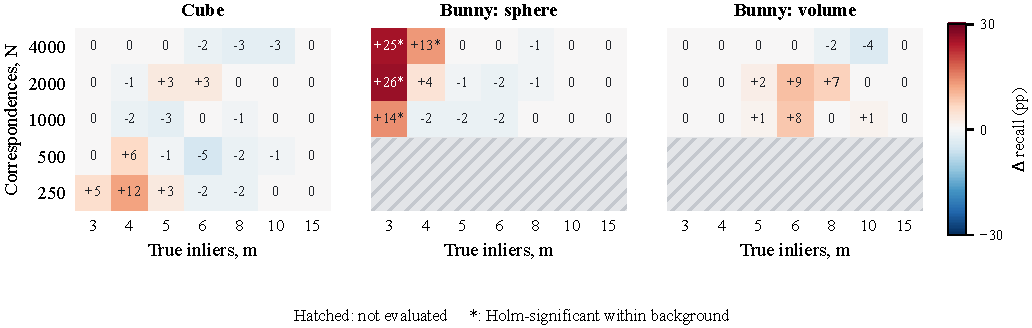
\includegraphics[width=.95\linewidth]{shared/figures/fig_s13.pdf}
\caption{Fresh synthetic inputs (100 per cell): \ngr{} minus the better of six baseline arms (three methods, two parameter sets each), in percentage points; red: \ngr{} higher. Stars: Holm-significant within a background; hatched cells were not evaluated. The sphere cells lose significance once MAC uses \ngr{}'s count readout.}
\label{S-fig:s-fresh}
\end{figure*}

\paragraph{Fresh-draw protocol.} We draw new inputs from the three benchmark generators using master seed 2026110301. \Cref{S-fig:s-fresh} has 77 cells of 100 inputs: $m\in\{3,4,5,6,8,10,15\}$ with $N\in\{250,500,1000,2000,4000\}$ on the cube background (35 cells, independent draws) and $N\in\{1000,2000,4000\}$ on the sphere and volume backgrounds, where inliers are sampled from the first 1000 Bunny vertices. For each of these backgrounds, the 21 cells share poses and source clouds and are nested in $N$ and $m$. Each baseline runs with both of its parameter sets, the original and the calibrated one, and \ngr{} is compared with the better of the six baseline arms in each cell (exact McNemar test, Holm over the cells of a background).

On these 7700 inputs, with each baseline given the better of its two parameter sets, \ngr{} is never significantly worse than the best baseline arm, with the largest gains on the most dilute inputs. With three inliers on the sphere background it registers 67, 48 and 29 of 100 inputs at $N=1000$, 2000 and 4000, against 53, 22 and 4 for the best baseline arm (Holm $p\le0.05$ in each cell). With four inliers at $N=4000$, the counts are 84 against 71. With three inliers, growth adds 5--10 inputs per cell and loses none ($+22/-0$ over the three cells), while summed over all cells its effect is smaller ($+86/-45$ on the cube background, $+19/-11$ on the volume and $+24/-22$ on the sphere; one of the 77 cells is significant after Holm correction). Part of the advantage comes from \ngr{}'s count readout: MAC equipped with it closes the sphere gaps (none of the six cells with three or four inliers is significant). Elsewhere, the frontends perform similarly. The cube advantage of the frozen benchmark does not reproduce with fresh seeds (62 against 63 for MAC with its original parameters).

\paragraph{Thinned real scans.} We also test low inlier counts with the outlier structure of real scans. From the FPFH correspondences of 3DMatch and 3DLoMatch, a pair is eligible if its first 5000 matches contain at least 20 true inliers and 2000 mismatches (residual below $\tau=0.1$\,m under the ground-truth pose; the ground truth is used only to build the input). This criterion admits 1478 of the 1623 3DMatch pairs and 1165 of the 1781 3DLoMatch pairs. The same seeded selection of 200 eligible pairs per benchmark is used in every cell: $m\in\{5,10,20\}$ true inliers and $N-m$ real mismatches with $N\in\{500,1000,2000\}$, nested (the five inliers are among the ten, the mismatches of $N=500$ among those of $N=1000$). Each frontend's native output is scored with the indoor criterion ($15^\circ$, 0.3\,m); finishing is not used. On these 18 cells of 200 pairs (Holm over the nine cells of each benchmark) no frontend is consistently ahead. On 3DMatch SC$^2$-PCR registers more pairs than \ngr{} in 8 of the 9 cells, significantly more than \ls{} with five inliers among 500 matches (84 against 63, $+29/-8$, $p=0.007$), and no difference involving \ngr{} is significant on either benchmark.

\subsection{Decoy clusters}

\begin{figure}[t]
\centering
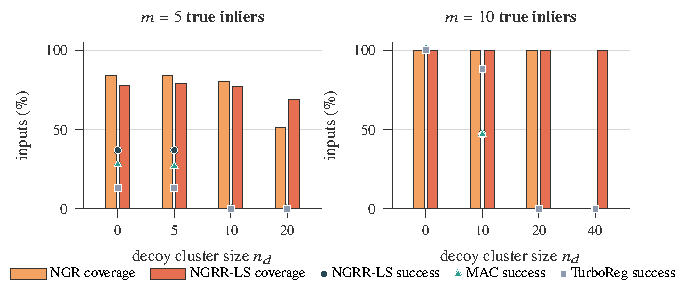
\includegraphics[width=\linewidth]{shared/figures/fig_s14.pdf}
\caption{Decoy clusters (cube, $N=1000$, 100 inputs per bar): $n_d$ outliers are replaced by matches of a second rigid motion. Bars: inputs whose refined candidates contain the true pose. Markers: final success of each frontend's own output (\ngr{} is within one input of \ls{}).}
\label{S-fig:s-decoy}
\end{figure}

Random outliers rarely form compatible clusters. Site capacity gives no significant gain on the cube benchmark above (169 against 173). \Cref{S-fig:s-decoy} plants a decoy on fresh cube inputs with $N=1000$ and $m\in\{5,10\}$: $n_d\in\{0,m,2m,4m\}$ outliers are replaced by matches of a second random rigid motion with the same noise, and the other outliers stay uniform; the baselines use their calibrated parameters. With ten inliers, a 40-match decoy captures every nucleus: the true pose is among \ngr{}'s candidates for 0 of 100 inputs and among \ls{}'s for 100 ($+100/-0$). With five inliers and a 20-match decoy, coverage rises from 51 to 69 ($+22/-4$, Holm $p=0.002$). With smaller decoys, capacity has little effect or slightly reduces coverage (78 against 84 for \ngr{} without a decoy, not significant). Final success is zero for every method once the decoy outnumbers the inliers, because correspondence consensus alone prefers the larger cluster. When the decoy and inlier sets have the same size, performance varies by method: with ten inliers TurboReg registers 88 inputs and \ngr{}, \ls{} and MAC 47 (\ngr{} against TurboReg $+1/-42$, $p=10^{-11}$); with five inliers \ngr{} registers 38, MAC 27 and TurboReg 13.
\FloatBarrier
\section{Nucleation crowding and diversity}
\label{S-sec:s-crowding}

We measure candidate crowding, correct-pose coverage among the first $k$ candidates (\cref{S-fig:s-crowding}b), and the cost and sensitivity of site capacity. Unless stated otherwise, the results use the training cohort of 3000 FPFH pairs from 82 3DMatch training scenes.

\begin{table*}[t]
\caption{Same-budget diversity controls on 3000 training pairs. Distinct and Cov.@1024 measure raw candidates; Ceiling measures the refined pool and Reg. the released result. Time is relative to NGRR-LS in this run.}
\label{S-tab:s-diversity}

\centering\small
\begin{tabular}{lrrrrr}
\toprule
Second half & Distinct $\uparrow$ & Cov.@1024 $\uparrow$ & Ceiling $\uparrow$ & Reg. $\uparrow$ & Time \\
\midrule
ranking (\ngr{}) & 222.6 & 2528 & 2429 & 2298 & -- \\
site capacity (\ls{}) & \textbf{409.6} & \textbf{2639} & \textbf{2487} & \textbf{2326} & 1.00 \\
MMR, $\lambda=\frac12$ & 337.8 & 2624 & \textbf{2487} & \textbf{2326} & 0.94 \\
hard capacity & 363.2 & 2615 & 2467 & 2312 & 0.90 \\
pose NMS & 243.0 & 2547 & 2438 & 2310 & 0.91 \\
\bottomrule
\end{tabular}

\end{table*}

\paragraph{The crowding statistic.} We diagnose crowding stage by stage on the training cohort. Ground truth is used to label candidates only after the frontend has run. True inliers are the matches whose residual under the ground-truth pose is below $\tau=0.1$\,m, and a triple is pure if all three of its matches are true inliers. For each pair, the stages of the original \ngr{} frontend are rerun unchanged. Among the 372 pairs with at most 25 true inliers, the 1024 kept nuclei contain a pure triple for 95 pairs, whereas a deeper ranking of 16\,384 triples contains one for 189. This ranking uses the same affinity $T_{abc}$ and the same per-block search over shortlisted pairs. The difference is consistent with crowding (\main{\cref*{sec:capacity}}), although this statistic alone does not establish the mechanism.

\begin{figure*}[t]
\centering
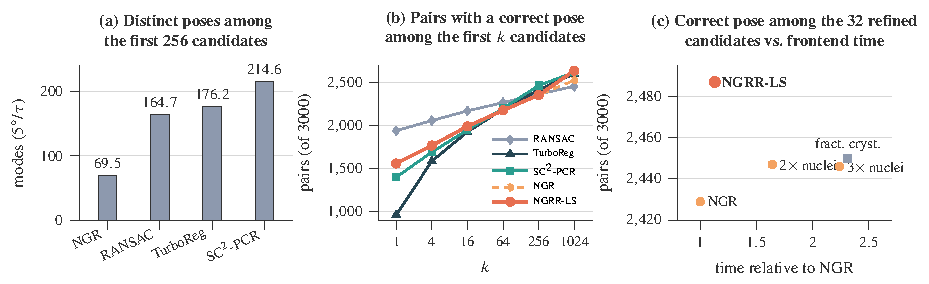
\includegraphics[width=.92\linewidth]{shared/figures/fig_crowding.pdf}
\caption[Nucleation crowding on the training cohort]{Nucleation crowding on the 3DMatch training cohort (3000 pairs, FPFH). (a) \ngr{}'s first 256 candidates contain few distinct poses; \ls{} keeps the same first half by construction. (b) Pairs with a correct pose among the first $k$ candidates before finishing: \ls{} departs from \ngr{} only beyond rank 256 and overtakes every baseline at 1024. (c) Pairs with a correct pose among up to 32 refined candidates against frontend run time, relative to \ngr{}: doubling or tripling the nuclei or fractional crystallization adds 17--21 pairs at 1.6--2.3$\times$ the time; the finite site capacity adds 58 at 1.13$\times$. Panels (a) and (c) are summarized in \main{\cref*{sec:crowding}}.}
\label{S-fig:s-crowding}
\end{figure*}

\paragraph{Crowding on the ranked candidates.} \ngr{}'s first 256 candidates contain only 69.5 distinct poses (greedy, at $5^\circ$ and $\tau$), a third of SC$^2$-PCR's 214.6; RANSAC has 164.7 and TurboReg 176.2. From rank 64 on, SC$^2$-PCR and TurboReg cover more pairs with a correct pose (\cref{S-fig:s-crowding}b; a candidate counts if it lies within $15^\circ$ and 0.3\,m of the ground truth, before finishing). Doubling or tripling the nucleus budget retains the original ranking and adds 18 and 17 pairs with a correct refined candidate, at 1.64$\times$ and 2.24$\times$ the frontend time. Fractional crystallization (harvesting the main crystal and renucleating from the depleted liquor) adds 21 at 2.31$\times$ the time. The finite site capacity raises coverage at rank 1024 from 2528 to 2639 pairs and the refined-pool ceiling from 2429 to 2487 ($+71/-13$, $p=8\times10^{-11}$), at 1.13$\times$ the run time. It was the only one of the four pre-registered candidate variants to pass the adoption rule; the doubled and tripled budgets were pre-registered as controls.

\paragraph{Test cohorts.} On the nine frozen test cohorts the ceiling rises from 10\,158 to 10\,292 pairs. The release assay converts this coverage gain into 9857 $\to$ 9920 registered pairs ($+121/-58$ paired, $p=3\times10^{-6}$). With the learned assay, the counts are 9969 $\to$ 10\,084 ($+199/-84$, $p=6\times10^{-12}$). The finishing step's anchor rule yields a smaller gain (9724 $\to$ 9752, $p=0.037$).

\paragraph{Site capacity against other diversity rules.} The controls in \cref{S-tab:s-diversity} keep \ls{}'s budget, first halves and deep rankings (65\,536 pairs, 16\,384 triples) and the same $K$, and fill the second halves using three alternative selection rules (defined in \cref{S-sec:s-method}). This comparison was added after the main evaluation; each rule was pre-registered before it was run, and the comparison does not change the reported pipeline. The columns of the table are: Distinct, the mean number of distinct poses ($5^\circ$, $\tau$) among the first 1024 candidates; Cov.@1024, pairs with a strictly correct pose among them; Ceiling, pairs with a correct pose among up to 32 refined candidates; Reg., pairs registered after finishing and the release assay; and Time, the mean frontend time relative to \ls{} in the same run. MMR is maximal marginal relevance on the match sets. The \ls{} row matches the pre-registered run (ceiling 2487).

Maximal marginal relevance, with its default trade-off $\lambda=\frac12$, reaches exactly the same ceiling as the site capacity (2487 pairs, $+16/-16$) and the same final count (2326, $+13/-13$), with fewer distinct poses (338 against 410 among the first 1024). A hard capacity (a match may sit in at most 8 pairs or 4 triples) runs out of admissible motifs in 1187 of the 3000 pairs and fills the remaining slots in ranking order. Its coverage is lower by 20 pairs ($+9/-29$, Holm $p=0.008$). Suppressing nuclei whose three-point pose repeats an earlier one loses 49 ($+10/-59$, Holm $p=8\times10^{-9}$) and only slightly increases the number of distinct poses (243, against 223 for \ngr{}): nuclei with different seed poses still grow into the same few modes. After verification the differences shrink (2312 and 2310 registered pairs against 2326; Holm $p=0.05$ and $0.08$). These controls support soft penalties on shared matches as a way to reduce crowding.

\paragraph{Cost and constants.} On the training cohort the site capacity adds 13\% to the frozen frontend time (mean time ratio 1.13), doubling the nuclei 64\%. These are mean ratios relative to \ngr{}, as in \cref{S-fig:s-crowding}c; the Time column of \cref{S-tab:s-diversity} is relative to \ls{} in the same run, and the median times in \main{\cref*{tab:joint}} come from 100 3DLoMatch+FPFH pairs. Halving or doubling either site-capacity constant changes the refined-pool ceiling and the final count on 1000 training pairs by at most three pairs. The capacities $q=8$ for pairs and $q=4$ for triples were fixed when the variant was pre-registered and never tuned.
\FloatBarrier
\section{Verification stages and release-rule calibration}
\label{S-sec:s-verification}

\begin{table*}[t]
\caption{Candidate recovery and conversion on all 1781 3DLoMatch+FPFH pairs. Native, winner-only ICP, finishing and release are recall (\%); $C$ is correct-pose coverage after the fixed finishing procedure. The gap $C-\mathrm{Native}$ is in percentage points, computed before rounding; $E$ is the percentage of covered pairs successfully released. Coverage uses ground truth only for diagnosis.}
\label{S-tab:s-utilization}
\centering
\small
\begin{tabular}{lrrrrrrr}
\toprule
Frontend & Native & Winner ICP & Finishing & Release & Coverage $C$ & $C-\mathrm{Native}$ & $E$ \\
\midrule
RANSAC-1M & 35.1 & 39.9 & 45.7 & 48.8 & 54.2 & 19.1 & 90.1 \\
SC$^2$-PCR & 39.0 & 42.2 & 49.7 & 52.6 & 59.8 & 20.8 & 87.9 \\
MAC & 40.0 & 43.2 & 49.4 & 51.6 & 59.7 & 19.8 & 86.4 \\
TurboReg & 38.5 & 41.8 & 49.0 & 51.5 & 56.4 & 18.0 & 91.3 \\
NGR & 40.3 & 42.8 & 48.7 & 51.1 & 56.4 & 16.1 & 90.6 \\
NGRR-LS & 40.4 & 43.0 & 49.6 & 53.1 & 59.2 & 18.8 & 89.8 \\
\bottomrule
\end{tabular}

\end{table*}

The native-to-refined-pool gap is 16.1--20.8 percentage points for each of the six frontends (\cref{S-tab:s-utilization}). Coverage measures the pool after prescribed allocation and refinement; those hypotheses need not have been correct in their coarse form. Backend timings are measured separately on a 100-pair subset at the specified CPU thread count.

\begin{figure*}[t]
\centering
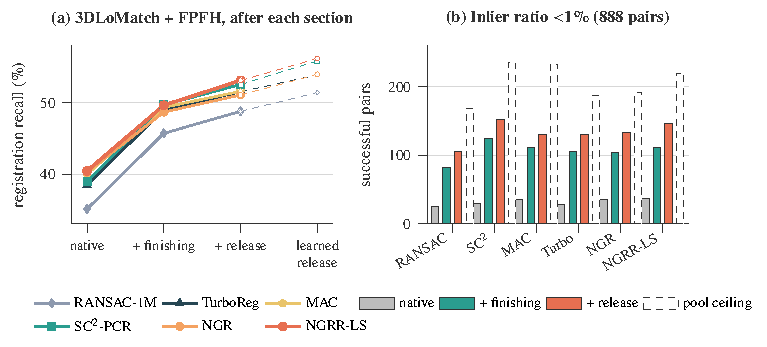
\includegraphics[width=.86\linewidth]{shared/figures/fig_results.pdf}
\caption[Recall after each section and on pairs below 1\% inliers]{(a) Recall on 3DLoMatch+FPFH after each section, for every frontend; dashed: the optional learned assay. (b) Pairs with an input inlier ratio below 1\% (888 of 1781): successes of the native output, after finishing, after the release assay, and the refined-pool ceiling. Panel (b) also appears as \main{\cref*{fig:dilute}}(a).}
\label{S-fig:s-results}
\end{figure*}

\paragraph{Recall after each stage.} \Cref{S-fig:s-results}a follows every frontend on 3DLoMatch+FPFH through finishing and release. Training-free verification raises recall by 10.8--13.7 percentage points for all six frontends, and the optional learned assay adds another 1.8--3.3 percentage points on 3DLoMatch with FPFH and FCGF. \Cref{S-fig:s-results}b isolates the 888 pairs with an inlier ratio below 1\%. The native frontends register 26--37 of them. Finishing raises this to 82--124, and the release assay to 106--152, 3.7--5.1 times the native count; the learned assay reaches 148--193 (not run for MAC). With the same verification SC$^2$-PCR releases the most of these pairs (152) and \ls{} 147.

\paragraph{Coverage and recall, unit by unit.} \main{\cref*{tab:joint}} reports stage gains and refined-pool conversion; \main{\cref*{tab:units}} isolates the generation controls. Coverage is the share of pairs whose refined pool, containing up to 32 candidates, includes a correct pose. Fixing the frontend and finishing procedure fixes this coverage; release selects within the resulting pool. Site capacity mainly changes coverage: on 3DLoMatch it adds 2.8 and 1.9 points of coverage with FPFH and FCGF (50 and 33 pairs), but changes the native output by only 0.1 and 0.2 points, and by at most 0.5 on any cohort. Finishing and release increase recall within that coverage: finishing adds 9.2 and 3.8 points and the release assay another 3.5 and 3.7, and the full verification procedure converts 89.8\% and 92.7\% of the coverage into registrations, close to the rate it achieves for \ngr{} (90.6\% and 93.7\%). The capacity's final gain on 3DLoMatch+FPFH (2.0 points, 36 pairs) thus comes from its coverage gain (50 pairs) processed by verification that converts both frontends' coverage at about the same rate; it reflects better candidate generation despite little change in the native output.

\paragraph{Finishing controls.} Refining only the native winner gives 43.0\% instead of 49.6\% (\ls, 3DLoMatch+FPFH). Refining the top 32 hypotheses with the same ICP and keeping the largest truncated correspondence support gives 32--72 fewer registered pairs than the finishing step for each of RANSAC, SC$^2$-PCR, MAC, TurboReg and \ngr{}; selecting by the highest Open3D fitness gives still lower recall (25.3--38.4\%).

\paragraph{Single-channel controls.} Over the nine cohorts, releasing by support alone or by residual shape alone gives 9760 and 9759 registered pairs with \ls{}, against 9920 for their minimum, and for every frontend the minimum releases more pairs than either channel alone.

\begin{table*}[t]
\caption[Release rules on the same refined pools]{Release rules on the same refined pools, limited to the first 32 candidates. Training: 12\,000 cells (3000 pairs, four frontends); test: 72\,117 cells (nine cohorts, every frontend where it completed; MAC's 3497 failed pairs are excluded). A cell succeeds if its selected candidate is correct. $s$, $h$: the normalized channels of the release assay (\main{\cref*{eq:assay}}, also in the first row); ties by $s$, $h$, queue order (lexicographic $s$-then-$h$ is equivalent to the $s$-only rule). Against \main{\cref*{eq:assay}}: test cells released by the rule but not by it and vice versa, and test pairs on which the rule releases more or fewer of the frontends' cells; the cells of one pair share its scans and correspondences, so $p$ is from a sign test over pairs, Holm-corrected over the seven rules. Bottom: the expected count of a uniform choice inside the non-dominated set, and bounds that no rule on these pools can exceed (the non-dominated set bounds every rule above).}
\label{S-tab:s-rules}
\centering\footnotesize
\begingroup
\let\origcref\cref
\renewcommand{\cref}[1]{\origcref{#1}}
\begin{tabular}{lrrrrr}
\toprule
Release rule & Training $\uparrow$ & Test $\uparrow$ & Cells & Pairs & Holm $p$ \\
\midrule
$\min(s,h)$ & 9209 & 58922 &  &  &  \\
support $s$ only & 8925 & 58020 & $+172/-1074$ & $+81/-399$ & $1\times10^{-50}$ \\
shape $h$ only & 8900 & 57812 & $+1021/-2131$ & $+362/-779$ & $6\times10^{-35}$ \\
$\lambda s+(1-\lambda)h$, $\lambda=0.3$ from training & \textbf{9290} & \textbf{59288} & $+624/-258$ & $+258/-112$ & $9\times10^{-14}$ \\
product $sh$ & 9208 & 58960 & $+140/-102$ & $+84/-62$ & 0.16 \\
harmonic mean & 9211 & 58964 & $+135/-93$ & $+81/-55$ & 0.10 \\
rank sum (Borda) & 9164 & 58806 & $+371/-487$ & $+190/-224$ & 0.16 \\
\midrule
uniform choice in the non-dominated set (expected) & & 58075 & & & \\
non-dominated set contains a correct pose & & 60311 & & & \\
pool contains a correct pose (ceiling) & 9754 & 61144 & & & \\
\bottomrule
\end{tabular}

\endgroup

\end{table*}

\subsection{Null calibration and alternative release rules}

The minimax-regret argument of \main{\cref*{sec:assay}} covers linear trade-offs between two normalized surrogates, not registration success, and the shape channel rests on a null that real scans need not satisfy. We test both on the stored refined pools of every frontend and cohort, with no new generation or refinement (\cref{S-tab:s-rules}). A cell is one frontend on one test pair. These comparisons were added after the main evaluation; each was pre-registered before it was run, and none changes the reported pipeline.

\paragraph{Null model and ranking.} For clearly wrong candidates (RE${}>30^\circ$ or TE above three times the success threshold) the null predicts $\bar u\approx\frac12$. We measure medians of 0.17--0.24 on the indoor cohorts and 0.28--0.33 on KITTI and ETH, and $\bar u<\frac12$ for at least 99.7\% of the wrong candidates in every cohort: wrong poses can also align planar patches, producing concentrated residuals. $\psi$ is therefore not a calibrated likelihood ratio. Correct candidates nevertheless have lower residual means (medians 0.12--0.18), and in pools containing both correct and incorrect candidates, the shape channel separates them with a pool-averaged AUC of 0.83--0.99, the support channel with 0.89--1.00, and their minimum with 0.89--1.00.

\paragraph{Alternative release rules.} The product and the harmonic mean of the two channels, also parameter-free, succeed on 38 and 42 more of the 72\,117 test cells than the release assay (0.05--0.06\%). These differences are not significant when tested over pairs (better on 84 and 81 pairs, worse on 62 and 55; Holm $p=0.16$ and $0.10$). Support alone and shape alone succeed on 902 and 1110 fewer cells, and a rank sum succeeds on 116 fewer (not significant by pair). A weighted sum whose one weight is chosen on the training cohort ($\lambda=0.3$) releases 366 more ($+624/-258$ cells; better on 258 pairs and worse on 112, Holm $p=9\times10^{-14}$), gains in eight of the nine cohorts (one tie), and raises \ls{} from 9920 to 9992 registered pairs over the nine cohorts. Learning the release from 26 features raises it to 10\,084. The minimax guarantee concerns surrogate trade-offs. For registration, two other parameter-free combinations perform similarly, one fitted weight improves success on about 0.5\% of cells, and the learned assay improves it further. We keep \main{\cref*{eq:assay}}, frozen before these comparisons, as the training-free default. Every rule here chooses inside the non-dominated set of the pool, which holds a correct candidate in 60\,311 of the 61\,144 cells whose pool does. A uniform choice inside it would release 58\,075.

\subsection{Allocation against plain Top-K at matched refinement budget}
\label{S-sec:s-topk}

This control was pre-registered before it was run and does not change the reported pipeline. Each cell is one frontend on one test pair. A is finishing's published allocated pool, with $n_i$ actual ICP calls. B is plain Top-K with exactly the same $n_i$ calls: it begins with the native winner, then takes the correspondence-support-ranked shortlist after the same $5^\circ$/$\tau$ suppression. When that shortlist is shorter than $n_i$, B fills the remaining calls with the next legal raw hypotheses in the same order. C refines the complete stored Top-K bank, up to 32 candidates. All three arms use the same SurfaceICP implementation and the same release rule of \main{\cref*{eq:assay}}. The support and shape channels use the same query points. Ground truth is read only after the final candidate has been selected.

The reproducibility checks all pass. A reproduces the published release in every cell. Recomputing A on the B/C evidence path reproduces its information scores to within $1.1\times10^{-15}$ and its residual moments exactly. The A and C coverage values match the stored records, every recomputed shortlist has the expected length, and the run contains no frontend errors.

Across nine test cohorts, A and B each make 1\,216\,817 ICP calls. A releases 58\,922 correct cells and B releases 58\,340, a paired difference of $+849/{-}267$ (\cref{S-tab:s-topk}; MAC's cells hold the pools of our earlier Python adaptation, and without them the main paper reports 51\,900 against 52\,372, $+693/{-}221$). Six correspondence frontends remain significant after Holm correction, with the largest adjusted $p$ value $8.9\times10^{-7}$. LGR has no significant difference ($+10/{-}7$, $p=0.63$). Cells from the same pair are not independent, so we also aggregate the A--B difference per point-cloud pair. A is better on 401 pairs and B on 150 ($p=2.1\times10^{-27}$). After grouping descriptor variants of the same scan pair, the result is 368 scan pairs versus 137 ($p=1.9\times10^{-25}$).

The mechanism is visible in the coverage and selection decomposition. A's refined pools contain a correct pose in 61\,144 cells, compared with 59\,784 for B, a gain of 1\,360 cells. The final gain is smaller because the fixed release rule selects 58\,922 of A's covered cells (96.37\%) and 58\,340 of B's covered cells (97.59\%). Allocation therefore improves candidate recovery. It does not raise conditional selection effectiveness under the fixed release rule. On 3DLoMatch+FPFH with \ls{}, A, B and C register 946, 907 and 908 of 1781 pairs, corresponding to 53.12\%, 50.93\% and 50.98\%.

C makes 1\,747\,401 ICP calls, 43.6\% more than A, and releases 58\,514 correct cells. This shows that the A--B difference is not explained by using more refined candidates. The control matches the number of ICP calls, not total wall-clock time. On the 100-pair 3DLoMatch+FPFH timing subset, the frozen implementation takes 2.45\,s per pair for A and 0.87\,s for B with SC$^2$-PCR. For TurboReg, the corresponding medians are 6.20\,s and 1.49\,s. The extra time comes from scoring candidates before ICP. The compiled finishing implementation used in the main timing table takes 0.09--0.11\,s per pair; a compiled B implementation was not measured.

\begin{table*}[t]
\centering
\footnotesize\setlength{\tabcolsep}{3pt}%
\begin{tabular}{lrrrrrrrr}
\toprule
& & \multicolumn{3}{c}{Released correct} & \multicolumn{2}{c}{A vs.\ B} & \multicolumn{2}{c}{ICP calls} \\
\cmidrule(lr){3-5}\cmidrule(lr){6-7}\cmidrule(lr){8-9}
Frontend & Cells & A & B & C & $+a/{-}b$ & Holm $p$ & A $=$ B & C \\
\midrule
RANSAC-1M & 12035 & 9771 & 9701 & 9729 & $+111/{-}41$ & $4\times10^{-8}$ & 179562 & 252148 \\
SC$^2$-PCR & 12035 & 9948 & 9885 & 9902 & $+109/{-}46$ & $9\times10^{-7}$ & 244190 & 367848 \\
MAC & 8538 & 6550 & 6440 & 6481 & $+156/{-}46$ & $2\times10^{-14}$ & 188278 & 273216 \\
TurboReg & 12035 & 9886 & 9746 & 9783 & $+186/{-}46$ & $3\times10^{-20}$ & 255238 & 385120 \\
LGR (GeoTr) & 3404 & 2990 & 2987 & 2990 & $+10/{-}7$ & 0.63 & 69221 & 108928 \\
NGR & 12035 & 9857 & 9753 & 9786 & $+140/{-}36$ & $7\times10^{-15}$ & 128805 & 158991 \\
\ls{} & 12035 & 9920 & 9828 & 9843 & $+137/{-}45$ & $2\times10^{-11}$ & 151523 & 201150 \\
\midrule
All & 72117 & 58922 & 58340 & 58514 & $+849/{-}267$ & -- & 1216817 & 1747401 \\
\bottomrule
\end{tabular}%

\caption{Allocation against plain Top-K over the nine test cohorts. A is finishing's allocated pool and reproduces the published release. B is plain Top-K with A's actual ICP calls on every cell. C is the full stored Top-K bank. All arms use the same ICP and release rule. $+a/{-}b$ gives cells registered by A but not B, and vice versa. The $p$ values are exact McNemar tests with Holm correction over the seven frontends. MAC: the pools of our earlier Python adaptation, only pairs within its resource limit (\cref{S-sec:s-maccpp}).}
\label{S-tab:s-topk}
\end{table*}

\subsection{Standard and published verification rules on the same pools}
\label{S-sec:s-selectors}

The comparison of the eight external rules was pre-registered before it was run; FS-TCD was added afterwards. Neither changes the reported pipeline. Every rule chooses one candidate inside the same refined pool as the release, so generation, allocation and ICP are identical; no ICP is re-run. A cell is one frontend on one test pair, as in \cref{S-tab:s-rules}; MAC's cells hold the stored pools of our earlier Python adaptation (\cref{S-sec:s-maccpp}). The main paper reports these comparisons without MAC's cells: release registers 52\,372 of 63\,579 cells, CorAl 51\,432 and prerejective 51\,376; matched Top-K 51\,900 ($+693/{-}221$) and full Top-32 52\,033 with 43.3\% more ICP calls; release 31\,064 against FS-TCD 29\,891 of 39\,590 cells ($+1654/{-}481$). Pool A is the finishing step's refined pool (its first 32 valid candidates). Pool C is the complete plain Top-K bank of \cref{S-sec:s-topk}.

\paragraph{Rules.} Five scores come from the finishing quantities or ICP: $M\sqrt G$, $M$, $G$, Open3D fitness with RMSE as tie-break, and a truncated Chamfer distance. Eight external training-free rules are our implementations of published verification scores on the voxelized observed clouds. LCP counts source points within $\delta$ of the target~\cite{aiger2008fpcs}, and OpenGR's weighted LCP~\cite{mellado2014super4pcs} weights them by a bisquare kernel. PCL's greedy verification~\cite{rusu2011pcl} subtracts $\lambda$ times the unexplained source points from the explained target points. The single-hypothesis GHV cost~\cite{aldoma2012ghv}, without occlusion reasoning, rewards normal-consistent explained points and penalizes outliers and clutter. SAC-IA~\cite{rusu2009fpfh} minimizes the truncated sum of distances. The prerejective score~\cite{buch2013prerejective} takes the smallest inlier mean squared distance among candidates whose inlier share is at least $g$. CorAl~\cite{adolfsson2021coral} minimizes the joint minus separate differential entropy of radius-$r$ neighborhoods, and MPV~\cite{razlaw2015mpv} minimizes the mean plane variance of the joint neighborhoods. Distances and radii are in units of $\tau$, and neighborhoods are exact. Each rule except SAC-IA has one parameter, chosen on the training cohort's pool A from a registered grid: $\delta=0.5$ for LCP and WLCP, $\lambda=0.5$, a GHV weight of 0.5, $g=0.1$, $r=3$ for CorAl and $r=2$ for MPV. With library-style defaults, prerejective registers 57\,780 cells and CorAl 56\,678. GT labels the chosen candidates only after every rule has chosen.

\paragraph{Results.} \Cref{S-tab:s-selector-full} lists every rule and \cref{S-tab:s-selector-cohort} the cohorts. Release registers 58\,922 cells on pool A and 58\,514 on pool C. The best external rules are CorAl with 57\,792 on pool A and prerejective with 56\,851 on pool C; with its default parameter, prerejective reaches 57\,780 on pool A. Every comparison favors release at the cell level (McNemar with Holm, $p\le9.8\times10^{-73}$, the largest for CorAl), over pairs and over scan pairs. Over pairs and scan pairs the weakest is prerejective, with 830 against 386 pairs ($p=8.5\times10^{-38}$) and 635 against 306 scan pairs ($p=3.3\times10^{-27}$). Overlap scores fail where overlap is low: on 3DLoMatch+FPFH, ICP fitness releases 2494 of 10\,686 cells, fewer than the frontends' native outputs. Against the best external rule of each cohort, the lead sums to 433 cells, two thirds of it on 3DLoMatch+FPFH. It is 287 cells on 3DLoMatch+FPFH and 81 on 3DMatch+FPFH, but at most 5 cells with FCGF on 3DMatch and 3DLoMatch, and 27 and 65 with GeoTransformer. On the saturated ETH and KITTI+FCGF cohorts, surface-overlap rules reach or nearly reach the ceiling (4175 and 2852 of 2854 cells), and release is within 28 and 6 cells. None of these rules reaches the 58\,075 cells of a uniform choice inside the non-dominated set of \cref{S-sec:s-verification}. The Python implementation of all eight external rules together takes a median of 170\,s per pair with exact neighborhoods. This is the cost of the experiment, not a speed comparison.

\paragraph{FS-TCD of SC$^2$-PCR++.} SC$^2$-PCR++~\cite{chen2023sc2pp} selects its model with a feature- and spatial-consistency constrained truncated Chamfer distance (FS-TCD). We port its \texttt{select\_best\_trans} and \texttt{post\_refinement} line by line from the official code (commit 5a654fd) to the CPU and apply it to the same pool A. The one-to-one matches are the cached correspondences, and the relaxed matches are each source point's 100 nearest target keypoints in descriptor space, as in the official matcher. The settings are those the official test scripts execute: inlier threshold 0.1\,m and FS-TCD threshold 0.05\,m indoors, 0.6\,m and 0.05\,m on KITTI. The rule needs keypoint descriptors, so it is evaluated on the six cohorts with descriptor archives. The cells are those of pool A above, and the recomputed release matches the published release in every cell. Unlike the official loaders, we use all cached keypoints without random subsampling. The KITTI configuration file lists an FS-TCD threshold of 0.1\,m, which gives 35\,133 cells in total. Release registers more cells in every cohort (\cref{S-tab:s-fstcd}), 36\,495 against 35\,102 of 46\,710 ($+1991/{-}598$, exact McNemar $p<10^{-170}$). Scoring each chosen candidate after its post-refinement, or never overwriting the one-to-one matches, gives 35\,210 and 35\,119 cells.

\begin{table}[t]
\caption{All selection rules on pool A, with pool C's count (\cref{S-sec:s-selectors}). Correct cells over the nine test cohorts. Pairs $+/{-}$: pairs on which release registers more or fewer of the frontends' cells than the rule.}
\label{S-tab:s-selector-full}
\centering
\footnotesize\setlength{\tabcolsep}{2.5pt}%
\begin{tabular}{@{}lrrrrr@{}}
\toprule
Rule on pool A & All & 3DLoMatch & Others & Pairs $+/{-}$ & Pool C \\
Cells & 72117 & 32674 & 39443 & & 72117 \\
\midrule
Release (ours) & 58922 & 21491 & 37431 & -- & 58514 \\
\midrule
$M\sqrt{G}$ & 57696 & 20575 & 37121 & $484/62$ & -- \\
$M$ & 56997 & 20405 & 36592 & $679/78$ & -- \\
$G$ & 51913 & 15370 & 36543 & $2064/237$ & -- \\
Truncated Chamfer & 51902 & 15330 & 36572 & $2076/242$ & -- \\
Fitness + RMSE & 49355 & 13621 & 35734 & $2801/190$ & -- \\
\midrule
CorAl~\cite{adolfsson2021coral} & 57792 & 21088 & 36704 & $1066/488$ & 55245 \\
Prerejective~\cite{buch2013prerejective} & 57704 & 20661 & 37043 & $830/386$ & 56851 \\
MPV~\cite{razlaw2015mpv} & 57287 & 21100 & 36187 & $1179/464$ & 54733 \\
GHV~\cite{aldoma2012ghv} & 54582 & 17661 & 36921 & $1503/284$ & 55711 \\
WLCP~\cite{mellado2014super4pcs} & 53848 & 16869 & 36979 & $1601/279$ & 55567 \\
LCP~\cite{aiger2008fpcs} & 52644 & 15916 & 36728 & $1875/245$ & 54883 \\
SAC-IA~\cite{rusu2009fpfh} & 51898 & 15327 & 36571 & $2070/231$ & 54398 \\
Greedy~\cite{rusu2011pcl} & 49441 & 13669 & 35772 & $2782/206$ & 52574 \\
\midrule
Ceiling & 61144 & 23106 & 38038 & & 60336 \\
\bottomrule
\end{tabular}%

\end{table}

\begin{table*}[t]
\caption{Selection rules on pool A by cohort (correct cells, all frontends). Bold: the most correct cells in the row, excluding the ceiling. Fitness and $M\sqrt G$ are from the finishing records, the other rules as in \cref{S-tab:s-selector-full}.}
\label{S-tab:s-selector-cohort}
\centering
\footnotesize\setlength{\tabcolsep}{3pt}%
\begin{tabular}{@{}lrrrrrrrrr@{}}
\toprule
Cohort & Cells & Release & $M\sqrt G$ & Fitness & CorAl & Prerej. & MPV & GHV & Ceiling \\
\midrule
3DM FPFH & 9719 & \textbf{8794} & 8635 & 7869 & 8651 & 8713 & 8539 & 8622 & 9149 \\
3DM FCGF & 9428 & \textbf{8918} & 8871 & 8264 & 8913 & 8880 & 8911 & 8619 & 9065 \\
3DM GeoTr & 9822 & \textbf{9402} & 9394 & 9259 & 9367 & 9359 & 9375 & 9329 & 9468 \\
3DLo FPFH & 10686 & \textbf{5511} & 5108 & 2494 & 5224 & 5178 & 5187 & 4199 & 6166 \\
3DLo FCGF & 10681 & \textbf{7102} & 6667 & 3813 & 7089 & 6832 & 7100 & 5357 & 7677 \\
3DLo GeoTr & 11307 & \textbf{8878} & 8800 & 7314 & 8775 & 8651 & 8813 & 8105 & 9263 \\
ETH FPFH & 4278 & 4147 & 4056 & 4166 & 3707 & 3915 & 3291 & \textbf{4175} & 4175 \\
KITTI FPFH & 3330 & \textbf{3324} & \textbf{3324} & \textbf{3324} & 3220 & \textbf{3324} & 3223 & \textbf{3324} & 3327 \\
KITTI FCGF & 2866 & 2846 & 2841 & \textbf{2852} & 2846 & \textbf{2852} & 2848 & \textbf{2852} & 2854 \\
\bottomrule
\end{tabular}%

\end{table*}

\begin{table}[t]
\caption{SC$^2$-PCR++'s FS-TCD selection against release on pool A of the six cohorts with descriptors (correct cells, all frontends). $+/{-}$: cells registered by release only and by FS-TCD only.}
\label{S-tab:s-fstcd}
\centering
\footnotesize\setlength{\tabcolsep}{3pt}%
\begin{tabular}{@{}lrrrrr@{}}
\toprule
Cohort & Cells & Release & FS-TCD & $+/{-}$ & Ceiling \\
\midrule
3DMatch+FPFH & 9719 & \textbf{8794} & 8728 & $221/155$ & 9149 \\
3DMatch+FCGF & 9428 & \textbf{8918} & 8826 & $147/55$ & 9065 \\
3DLoMatch+FPFH & 10686 & \textbf{5511} & 5026 & $692/207$ & 6166 \\
3DLoMatch+FCGF & 10681 & \textbf{7102} & 6479 & $803/180$ & 7677 \\
KITTI+FPFH & 3330 & \textbf{3324} & 3246 & $79/1$ & 3327 \\
KITTI+FCGF & 2866 & \textbf{2846} & 2797 & $49/0$ & 2854 \\
\midrule
All six & 46710 & \textbf{36495} & 35102 & $1991/598$ & 38238 \\
\bottomrule
\end{tabular}%

\end{table}
\FloatBarrier
\section{Full real-scan results and qualitative cases}
\label{S-sec:s-results}

\begin{table*}[t]
\caption[Registration recall on nine test cohorts]{Registration recall (\%) on nine test cohorts, including GeoTransformer and ETH inputs beyond \main{\cref*{tab:main}}. ``native'': each frontend's own output. ``F+R'': common training-free verification with finishing of up to 32 candidates followed by the release assay of \main{\cref*{eq:assay}}. Bottom, ``+ learned release'': the optional learned assay, trained on 3DMatch-train. Bold: best and underlined: second best value of the column within each block, at the displayed precision. MAC is the authors' C++ code (\cref{S-sec:s-maccpp}); --: no released ETH setting, and the learned assay was not run on its pools. Each frontend has 16\,GiB and 600\,s per pair, and resource failures count as unregistered pairs. All frontends use the same inputs; the correspondence-based ones run on CPU. \ngr{} and \ls{} are ours, without and with the finite site capacity.}
\label{S-tab:s-main}
\centering\footnotesize
\setlength{\tabcolsep}{4pt}
\ifdefined\supptablebox\else\newsavebox{\supptablebox}\fi
\sbox{\supptablebox}{\begin{tabular}{llrrrrrrrrr}
\toprule
 & & \multicolumn{3}{c}{3DMatch} & \multicolumn{3}{c}{3DLoMatch} & ETH & \multicolumn{2}{c}{KITTI} \\
\cmidrule(lr){3-5}\cmidrule(lr){6-8}\cmidrule(lr){9-9}\cmidrule(lr){10-11}
Frontend & Output & FPFH & FCGF & GeoTr & FPFH & FCGF & GeoTr & FPFH & FPFH & FCGF \\
 & Pairs & 1623 & 1623 & 1623 & 1781 & 1781 & 1781 & 713 & 555 & 555 \\
\midrule
RANSAC-1M & native & 82.3 & 92.5 & \underline{95.4} & 35.1 & 57.9 & 77.4 & 55.8 & \underline{99.6} & \textbf{97.3} \\
 & F+R & 90.2 & \textbf{94.9} & 95.6 & 48.8 & \textbf{67.1} & 78.9 & 89.6 & \textbf{99.8} & \textbf{99.5} \\
\addlinespace[2pt]
SC$^2$-PCR & native & \textbf{83.7} & 92.9 & \textbf{95.6} & 39.0 & 58.3 & 78.1 & \textbf{78.5} & 99.5 & \underline{95.9} \\
 & F+R & \textbf{91.0} & \textbf{94.9} & \underline{96.1} & \underline{52.6} & \underline{67.0} & \textbf{80.3} & \textbf{99.2} & \textbf{99.8} & \underline{99.3} \\
\addlinespace[2pt]
MAC & native & 83.0 & \textbf{93.5} & \textbf{95.6} & 40.0 & \underline{59.0} & \underline{78.3} & -- & \underline{99.6} & 95.7 \\
 & F+R & 90.4 & \underline{94.8} & \textbf{96.2} & 51.6 & 66.4 & \underline{80.2} & -- & \textbf{99.8} & 98.9 \\
\addlinespace[2pt]
TurboReg & native & \textbf{83.7} & \underline{93.3} & \underline{95.4} & 38.5 & 58.7 & 77.9 & 75.9 & \textbf{99.8} & 95.5 \\
 & F+R & 90.4 & \underline{94.8} & \underline{96.1} & 51.5 & 66.1 & 79.8 & 98.0 & \textbf{99.8} & \textbf{99.5} \\
\addlinespace[2pt]
LGR (GeoTr) & native & -- & -- & \underline{95.4} & -- & -- & 77.3 & -- & -- & -- \\
 & F+R & -- & -- & \underline{96.1} & -- & -- & \textbf{80.3} & -- & -- & -- \\
\addlinespace[2pt]
NGR & native & \underline{83.4} & 92.9 & \underline{95.4} & \underline{40.3} & \underline{59.0} & 78.2 & \underline{78.1} & \textbf{99.8} & 95.3 \\
 & F+R & 90.3 & 94.5 & 96.0 & 51.1 & 65.7 & 79.4 & 98.3 & \textbf{99.8} & \underline{99.3} \\
\addlinespace[2pt]
NGRR-LS & native & \underline{83.4} & 93.2 & \textbf{95.6} & \textbf{40.4} & \textbf{59.2} & \textbf{78.6} & \underline{78.1} & \underline{99.6} & 95.3 \\
 & F+R & \underline{90.5} & \textbf{94.9} & 96.0 & \textbf{53.1} & 66.7 & 79.1 & \underline{98.7} & \textbf{99.8} & \textbf{99.5} \\
\midrule
\multicolumn{11}{l}{\emph{Optional learned assay (trained on 3DMatch-train only)}} \\
RANSAC-1M & learned release & 91.9 & 94.9 & 95.6 & 51.4 & \underline{69.5} & 78.8 & 89.8 & \textbf{99.8} & \textbf{99.6} \\
SC$^2$-PCR & learned release & \underline{92.4} & 95.2 & \textbf{96.4} & \underline{55.9} & \textbf{70.2} & \underline{81.1} & \textbf{99.9} & \textbf{99.8} & \textbf{99.6} \\
MAC & learned release & -- & -- & -- & -- & -- & -- & -- & -- & -- \\
TurboReg & learned release & \underline{92.4} & \underline{95.3} & \underline{96.2} & 53.9 & 68.1 & 80.6 & 98.6 & \textbf{99.8} & \underline{99.5} \\
LGR (GeoTr) & learned release & -- & -- & 96.0 & -- & -- & \textbf{81.4} & -- & -- & -- \\
NGR & learned release & 91.3 & 94.5 & 96.0 & 54.0 & 67.5 & 80.0 & 98.7 & \textbf{99.8} & \underline{99.5} \\
NGRR-LS & learned release & \textbf{92.5} & \textbf{95.4} & \underline{96.2} & \textbf{56.2} & 69.1 & 80.1 & \underline{99.3} & \textbf{99.8} & \underline{99.5} \\
\bottomrule
\end{tabular}
}%
\ifdim\wd\supptablebox>\textwidth\resizebox{\textwidth}{!}{\usebox{\supptablebox}}\else\usebox{\supptablebox}\fi

\end{table*}

\paragraph{The authors' C++ MAC.}\label{S-sec:s-maccpp} The MAC results of \main{\cref*{tab:joint,tab:main}}, \main{\cref*{fig:dilute,fig:pareto}} and \cref{S-tab:s-utilization,S-fig:s-results,S-tab:s-main,S-tab:s-cost} use the authors' C++ code with the 12 OpenMP threads it fixes, the same first $\le$5000 correspondences, the 16\,GiB/600\,s limits and the dataset settings of its release, which has none for ETH. On KITTI+FPFH, 25 pairs exceed 16\,GiB; rerun with higher limits, all of them complete (at most 116\,GiB and 1276\,s), so MAC has no unregistered pair from resource limits. Its pool is every hypothesis that MAC computes from its selected cliques, and the common finishing and release are applied unchanged; on 60 evenly spaced 3DLoMatch+FPFH pairs this backend reproduces the stored release of SC$^2$-PCR, with identical poses. The completed width-matched C++ run supplies the frozen synthetic figure and its count-readout control. Our earlier Python adaptation remains in \cref{S-sec:s-synthetic} for decoys, fresh draws and thinned real scans, in the stored pools of \cref{S-sec:s-verification} (release-rule calibration, Top-K and selection-rule comparisons; the main paper reports the latter two without MAC's cells), and in the MAC column of \cref{S-fig:s-qualitative}. Where both complete within the limits (3DMatch+FPFH, 3DLoMatch+FPFH and 3DLoMatch+FCGF), the two implementations register natively within 1.1 points of each other (83.0 against 81.9, 40.0 against 40.4 and 59.0 against 58.8\%). With matched compatibility settings, the checked outcomes agree: on three checked synthetic inputs it gives the same graph, maximal cliques and selected cliques as the authors' code, and on 300 of 300 inputs the same outcome. The authors' code sets this width from the mean point spacing of the clouds it receives, which on the sparse synthetic correspondence sets is about $1.83\tau$, $6.05\tau$ and $0.96\tau$ on cube, sphere and volume, respectively, instead of $0.75\tau$; this explains the lower automatic-scale synthetic recall. The frozen 750-input figure uses the width-matched C++ run; fresh draws, decoys and thinned real scans retain the Python adaptation.

\begin{table*}[t]
\caption[Official criterion]{GeoTransformer's official criterion (registration recall \%, scene mean) on its own correspondences. ``+ finishing'': the finishing step's own choice among up to 32 refined candidates; ``+ release'': the training-free release assay; ``+ learned release'': the optional learned assay. Bold: best per column.}
\label{S-tab:s-official}
\centering\footnotesize
\setlength{\tabcolsep}{4pt}
\begin{tabular}{lrrrrrrrr}
\toprule
 & \multicolumn{4}{c}{3DLoMatch (1726 pairs) $\uparrow$} & \multicolumn{4}{c}{3DMatch (1279 pairs) $\uparrow$} \\
\cmidrule(lr){2-5}\cmidrule(lr){6-9}
Frontend & native & + finishing & + release & + learned release & native & + finishing & + release & + learned release \\
\midrule
RANSAC-1M & 73.55 & 74.49 & 74.55 & 74.58 & 91.50 & 91.90 & 91.93 & 91.90 \\
SC$^2$-PCR & \textbf{74.36} & 75.01 & \textbf{76.02} & 76.35 & \textbf{92.63} & 92.67 & 93.09 & 93.07 \\
TurboReg & 73.57 & 75.15 & 75.93 & 76.42 & 92.09 & 92.59 & 93.09 & 92.64 \\
LGR (GeoTr) & 74.03 & \textbf{75.25} & 75.77 & \textbf{76.51} & 92.48 & \textbf{93.63} & \textbf{93.34} & 93.13 \\
NGR & 74.10 & 74.48 & 75.02 & 75.72 & 92.42 & 92.46 & 92.97 & 92.92 \\
NGRR-LS & 74.33 & 74.56 & 74.84 & 75.83 & 92.30 & 92.62 & 93.10 & \textbf{93.26} \\
\bottomrule
\end{tabular}


\end{table*}

\begin{figure*}[tp]
\centering
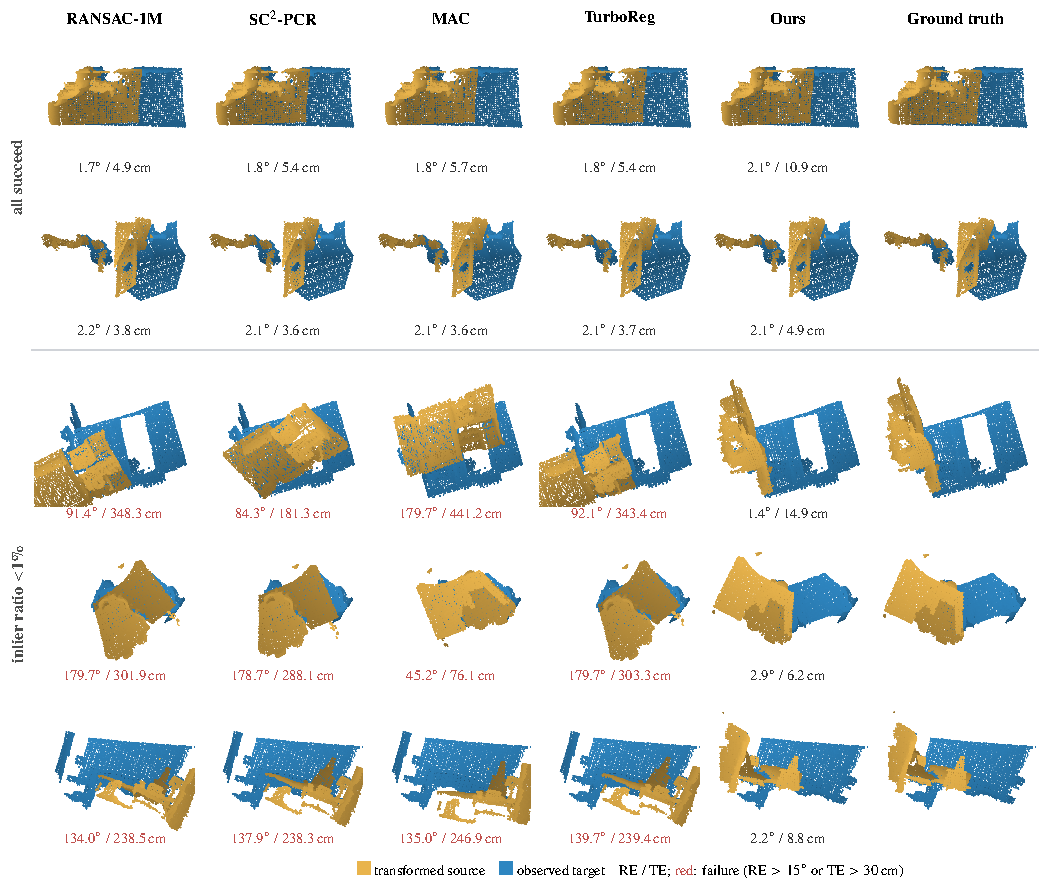
\includegraphics[width=\linewidth]{shared/figures/fig_qualitative.pdf}
\caption[Real cases]{Real cases on 3DLoMatch+FPFH. Gold: source transformed by each method's pose; blue: observed target; one camera and scale per row. Columns 1--4 are each frontend's native output, ``Ours'' is \ls{} with finishing and the training-free release assay. Rows were selected by outcome with a rule fixed before rendering: top, pairs that every method registers (563 pairs), ranked by the number of true inliers; bottom, pairs with an inlier ratio below 1\% on which all four baselines fail and ours succeeds (93 pairs with the earlier MAC adaptation shown in this figure; 97 with the C++ MAC), ranked by target size. Two and three rows were picked for legibility from the first four and six of each list (positions 1 and 2 of the first list; 1, 5 and 6 of the second).}
\label{S-fig:s-qualitative}
\end{figure*}

\paragraph{Paired comparisons.} In \cref{S-tab:s-main}, paired counts $+a/{-}b$ give the pairs registered by the first method but not by the second, and the reverse; $p$ is from McNemar's test~\cite{mcnemar1947}.

On 3DLoMatch+FPFH training-free verification raises recall by 10.8--13.7 percentage points for all six frontends, on 3DLoMatch+FCGF by 6.7--9.2, and on ETH, unseen during design, from 55.8--78.5\% to 89.6--99.2\%. On the saturated cohorts (3DMatch+GeoTr, KITTI+FPFH) the gains stay below one point. No frontend's recall decreases on any cohort.

With the same verification, \ls{} reaches 53.1\% on 3DLoMatch+FPFH, against 52.6\% for SC$^2$-PCR and 51.6\% for MAC. The paired difference from SC$^2$-PCR is not significant (+42/$-$32, $p=0.30$); against MAC it is +55/$-$28 ($p=0.004$). In contrast, \ls{} registers more pairs than \ngr{} (+45/$-$9), TurboReg and RANSAC-1M ($p\le10^{-3}$). On the other FPFH and FCGF cohorts it is within 0.5 points of the best frontend, and over the five frontends evaluated on all nine cohorts its total (9920 pairs) is second to SC$^2$-PCR (9948; +85/$-$113, $p=0.055$).

The optional learned assay adds 1.8--3.3 percentage points on 3DLoMatch with FPFH and FCGF and reaches 56.2\% with \ls{} on 3DLoMatch+FPFH (it was not run on the C++ MAC pools). We selected its features, regularization and weights using only the training cohort, but the 26 candidate features had been listed before the protocol was in place (\cref{S-sec:s-protocol}); we report it separately from the training-free results. Summed over the nine cohorts, the training-free assay obtains 50--58\% of the learned assay's gain over the finishing step's anchor rule for each of the five frontends. Over the nine cohorts, releasing by support alone or by residual shape alone gives 9760 and 9759 registered pairs with \ls{}, against 9920 for their minimum, and for every frontend the minimum releases more pairs than either channel alone.

\paragraph{Scene bootstrap.} Paired gains are more stable than absolute recall, which is estimated from only eight test scenes. A scene bootstrap (2000 resamples of the eight 3DLoMatch test scenes; 95\% intervals) gives 53.1\% [43.9, 60.4] for \ls{} on 3DLoMatch+FPFH, but a gain over its native output of 12.7 [10.3, 14.1] points and over \ngr{} of 2.0 [1.5, 2.5]; against SC$^2$-PCR the difference is 0.6 [$-0.3$, 1.6].

\paragraph{Extremely dilute pairs.} \Cref{S-fig:s-results}(b) and \main{\cref*{fig:dilute}}(a) isolate the 888 3DLoMatch+FPFH pairs with an inlier ratio below 1\%. The native frontends register 26--37 of them. Finishing raises this to 82--124, and the release assay to 106--152, 3.7--5.1 times the native count; the learned assay reaches 148--193 (not run for MAC). With the release assay SC$^2$-PCR registers the most of these pairs (152, against 147 for \ls{}), and the refined pools of the six frontends contain a correct candidate for 169--235 of them. The 381 pairs with only 11--25 true inliers among up to 5000 matches show the same pattern: 7--8 native, 32--38 after finishing and 39--51 after the release assay, where \ls{} registers the most (51). On the 250 pairs with at most ten true inliers every method stays near the floor (3--4 successes without learning, 6--10 with the learned assay).

\paragraph{Qualitative cases.} \Cref{S-fig:s-qualitative} shows real cases. When inliers are plentiful, the methods converge to the same pose. Below 1\% the baselines return poses that are off by 45--180$^\circ$ in the rows shown, while the full pipeline releases a correct candidate. In this cohort 563 pairs are registered by every method, and 93 pairs below 1\% by ours but by none of the four baselines' native outputs (97 with the C++ MAC of \main{\cref*{fig:dilute}}); the illustrations come from these two groups, and the counts above provide the aggregate comparison. The baselines are shown with their native outputs; \cref{S-tab:s-main} and \cref{S-fig:s-results}(b) give their counts with the same verification.

\paragraph{Official criterion.} \Cref{S-tab:s-official} uses GeoTransformer's official criterion (scene mean) on 1726 3DLoMatch and 1279 3DMatch pairs. Its own estimator LGR obtains 74.03\% on 3DLoMatch in our run (74.0\% in~\cite{qin2022geotransformer}); finishing and the release assay raise it to 75.77\%, and the learned assay to 76.51\%. The training-free verification improves every frontend, by 0.5--2.4 percentage points on 3DLoMatch and 0.4--1.0 on 3DMatch. On these learned correspondences, final recall differs by at most 1.5 points across frontends, and \ls{} is not among the best.

\paragraph{Further methods on the same inputs.} \main{\Cref*{tab:main}} adds SC$^2$-PCR++~\cite{chen2023sc2pp}, Regor~\cite{zhao2025regor} and DualReg~\cite{li2026dualreg}, run with their authors' code and per-dataset settings on the same first $\le$5000 correspondences, together with the registration recall and the rotation and translation errors of every frontend. SC$^2$-PCR++ and Regor receive the official keypoint descriptors for their feature-based steps, and DualReg the observed clouds with normals that we estimate from ten nearest neighbors, because the released normals belong to other correspondences; its recall on our inputs is below the published one (37.4 against 41.66\% on 3DLoMatch+FPFH, 94.1 against 98.20\% on KITTI+FPFH). On every cohort the complete pipeline registers at least as many pairs as these three methods, with a lower mean rotation error on the registered pairs.

The complete RR/RE/TE and timing table is in \main{\cref*{tab:main}}. SC$^2$-PCR++ full-cohort accuracy was measured on GPU, while its displayed 0.71\,s is from a separate 16-thread CPU run. On the same 100-pair timing subset the CPU and GPU runs register 45 and 43 pairs, respectively; Its mixed-device point is excluded from the CPU Pareto frontier. Regor uses GPU for both measurements. DualReg timing excludes normal estimation (median 0.026\,s); final release selection adds milliseconds beyond the timed moments.
\FloatBarrier
\section{Published numbers}
\label{S-sec:s-literature}
\main{\cref*{tab:literature}} lists recall as reported by 15 other methods. The locally run native baselines stay close to their published results (MAC 39.98\% against 40.88\% on 3DLoMatch+FPFH, SC$^2$-PCR 38.97\% against 38.57\%), which suggests that our inputs follow the standard protocol. On 3DLoMatch+FPFH the highest published numbers we found are 46.77\% (MAC-OP~\cite{yang2024mac}, which adds an overlap prior; reported second-hand) and 45.76\% (SVC~\cite{zhang2024svc}, which also reads the point clouds); Regor~\cite{zhao2025regor} reports 43.96\%. The training-free pipeline reaches 53.12\%. Our verification uses observed point clouds, so surface-using methods are the appropriate comparison group.

Asterisked entries come from the comparison tables of MAC~\cite{zhang2023mac} (TEASER++, SC$^2$-PCR on 3DLoMatch+FPFH and PointDSC on 3DLoMatch), SVC~\cite{zhang2024svc} (SC$^2$-PCR++ on 3DLoMatch+FPFH), HyperGCT~\cite{zhang2025hypergct} (VBReg on 3DLoMatch+FPFH and Hunter on 3DLoMatch+FCGF) and Regor~\cite{zhao2025regor} (the other Hunter entries). FastMAC uses its @50 configuration, TurboReg 2K indoors and 0.25K on KITTI, and PointDSC's KITTI values use models retrained on KITTI. Every number was checked against the source PDF; the five SC$^2$-PCR++ entries match the SC$^2$-PCR++ authors' release and the papers that compare against it.
\FloatBarrier
\section{Cost and the compiled implementation}
\label{S-sec:s-cost}

\begin{table}[t]
\caption[Run time on 3DLoMatch+FPFH]{Median seconds per pair on an AMD EPYC 9655P, using the same 100 3DLoMatch+FPFH inputs. Each thread count runs all frontends except MAC$^\dagger$ sequentially in one job on one node, from the same code version. All rows use compiled finishing, with Open3D's point-to-plane ICP and Tukey weighting implemented in compiled loops and exact surface queries below $\tau$; the frozen finishing implementation takes 2.3\,s with \ls{} at four threads. Total includes the frontend, finishing and release moments; final selection takes additional milliseconds. Rows marked Compiled use compiled frontend kernels with growth restricted to each phase's initial support (\cref{S-sec:s-cost}). The dense switch in \cref{S-tab:s-cohortcost} does not engage on these pairs. The measured outcomes match the frozen implementation. SC$^2$-PCR and MAC use their authors' code, and TurboReg its author core. $^\dagger$The authors' C++ MAC fixes 12 OpenMP threads; it is timed only at 16 threads, in a later job on the same node, where rerun NGRR-LS and SC$^2$-PCR reproduce their times within 5\%. \main{\cref*{tab:main}} gives the 16-thread accuracy--time summary.}
\label{S-tab:s-cost}
\centering\footnotesize
\setlength{\tabcolsep}{4pt}
\ifdefined\supptablebox\else\newsavebox{\supptablebox}\fi
\sbox{\supptablebox}{\begin{tabular}{lrrrrrrr}
\toprule
 & \multicolumn{3}{c}{4 threads} & & \multicolumn{3}{c}{16 threads} \\
\cmidrule(lr){2-4}\cmidrule(lr){6-8}
Frontend & Frontend & Finishing & Total & & Frontend & Finishing & Total \\
\midrule
RANSAC-1M & 0.50 & 0.13 & 0.62 & & 0.44 & 0.10 & 0.54 \\
SC$^2$-PCR & 1.18 & 0.11 & 1.30 & & 0.83 & 0.09 & 0.92 \\
MAC$^\dagger$ & -- & -- & -- & & 1.55 & 0.11 & 1.68 \\
TurboReg & 2.72 & 0.17 & 2.91 & & 1.84 & 0.11 & 1.96 \\
\ngr{} & 4.03 & 0.13 & 4.17 & & 1.57 & 0.09 & 1.67 \\
\ls{} & 4.20 & 0.12 & 4.34 & & 1.73 & 0.09 & 1.82 \\
\midrule
\ngr{}, compiled & 0.65 & 0.13 & 0.78 & & 0.29 & 0.10 & 0.38 \\
\ls{}, compiled & 0.65 & 0.12 & 0.78 & & 0.30 & 0.09 & 0.39 \\
\bottomrule
\end{tabular}
}%
\ifdim\wd\supptablebox>\columnwidth\resizebox{\columnwidth}{!}{\usebox{\supptablebox}}\else\usebox{\supptablebox}\fi

\end{table}

\begin{table}[t]
\caption[Run time per cohort]{Median seconds per pair of the frozen and compiled \ls{} frontends and of the compiled finishing step on the first 100 pairs of each test cohort, at four threads; both implementations run one after the other in one job per cohort (jobs may share a node). Ratio: frozen over compiled frontend. The compiled frontend uses the frozen dense products where supports exceed 1600 matches or 70\% of the candidates are non-negligible (\cref{S-sec:s-cost}). These are separate runs from \cref{S-tab:s-cost}, so 3DLoMatch+FPFH differs slightly.}
\label{S-tab:s-cohortcost}
\centering\footnotesize
\setlength{\tabcolsep}{4pt}
\begin{tabular}{lrrrr}
\toprule
 & \multicolumn{3}{c}{\ls{} frontend} & \\
\cmidrule(lr){2-4}
Cohort & Frozen & Compiled & Ratio & Finishing \\
\midrule
3DMatch+FPFH & 3.74 & 0.65 & 5.7$\times$ & 0.11 \\
3DLoMatch+FPFH & 4.53 & 0.71 & 6.4$\times$ & 0.15 \\
KITTI+FPFH & 1.30 & 0.40 & 3.3$\times$ & 0.15 \\
ETH+FPFH & 4.59 & 0.63 & 7.2$\times$ & 0.19 \\
\midrule
3DMatch+FCGF & 4.27 & 2.32 & 1.8$\times$ & 0.09 \\
3DLoMatch+FCGF & 4.60 & 1.05 & 4.4$\times$ & 0.13 \\
KITTI+FCGF & 5.07 & 3.41 & 1.5$\times$ & 0.15 \\
3DMatch+GeoTr & 5.24 & 3.66 & 1.4$\times$ & 0.09 \\
3DLoMatch+GeoTr & 3.54 & 2.34 & 1.5$\times$ & 0.09 \\
\bottomrule
\end{tabular}


\end{table}

\paragraph{Locality and the compiled frontend.} \Cref{S-tab:s-cost} times every frontend at four and sixteen threads, each thread count in one job on one node. In the frozen \ls{} frontend, which is among the slowest implementations in this comparison, two dense products account for about 70\% of runtime: growth of 1024 phases and triplet scoring. Both products are local on 3DLoMatch+FPFH.

After growth, all but $10^{-6}$ of a phase's weight lies on a median of 100--190 out of up to 5000 matches (380--600 initially). A triplet score is non-negligible only for matches compatible with both members of its pair. Our compiled implementation grows each phase on its initial support: matches holding at least $10^{-6}$ of the largest initial weight. It gathers the block once for all phases of a seed pair. It forms each triplet score from the compatible matches only (terms below $10^{-9}$ of the pair's largest common weight and compatibilities below $10^{-10}$ are dropped) and scores candidates in the order of an upper bound, so that each batch's 3072 best are found without scoring the rest. The remaining steps run in compiled loops, and the libraries for the pair supports and the $3\times3$ SVDs are unchanged. This support-restricted implementation of \main{\cref*{sec:method}} runs on CPU. The \ls{} frontend then takes 0.65\,s at four threads and 0.30\,s at sixteen, against 1.18\,s and 0.83\,s for SC$^2$-PCR's released implementation.

\paragraph{Learned correspondences and the dense switch.} Learned correspondences have larger supports: on the FCGF and GeoTransformer cohorts of 3DMatch and 3DLoMatch, the initial supports cover a median of 24--99\% of the matches (ten pairs each). Gathering these blocks for each seed pair costs more than using dense products. The compiled frontend therefore keeps the frozen dense growth when a pair's initial supports average more than 1600 matches, and the frozen dense triplet scores when more than 70\% of the candidates of its first 64 shortlisted pairs are non-negligible. Both switch points were set on 30 calibration pairs per cohort, none of them among the timed pairs. On these 300 pairs, the switch takes 0.4\% more time than choosing the faster product for every pair. Moving the thresholds within 1500--1700 matches and 65--75\% adds at most 1.1\,s to the 415\,s. The switch never engages on 3DLoMatch+FPFH, KITTI+FPFH and ETH, grows densely on 1--5\% of the other FPFH pairs, and on 10--99\% of the learned-descriptor pairs. With it, the compiled frontend is 3.3--7.2 times faster than the frozen one on the four FPFH cohorts (0.40--0.71\,s at four threads) and 1.4--4.4 times faster on the five learned-descriptor cohorts (1.05--3.66\,s; \cref{S-tab:s-cohortcost}), where most of the time stays in the same dense products.

\paragraph{Same outcomes, different pools.} With compiled verification and the dense switch, \ls{} matches the frozen pipeline's outcomes on all 15\,035 pairs of the training cohort and the nine test cohorts (the same success or failure of the native output, the refined-pool ceiling, the finishing step's choice and the released candidate). The compiled \ngr{} also matches these outcomes on the 4781 pairs of the training cohort and 3DLoMatch+FPFH. Compiled triplet scoring selects different nuclei, so the candidate pools differ. Sparse-matrix kernels inside the dense products were slower than the dense products, since 7--17\% of the weights stay above any useful threshold. No two phases coincide, so duplicate merging saves no work.

\paragraph{Compiled verification.} All frontends share the same verification implementation. Surface evidence uses only nearest-neighbor distances below $\tau$, because larger distances contribute zero. A grid with that cell size therefore answers the queries exactly from 27 cells. ICP and greedy suppression run in compiled loops. The ICP reproduces Open3D's \texttt{registration\_icp} iterations: on 829 calls, every stage found the same number of correspondences and poses differed by at most $4\times10^{-6}$ degrees. Other nearest-neighbor queries use several threads, correspondence scoring runs in a compiled loop, and residual moments are computed in place. The resulting success/failure outcomes match the frozen implementation on every checked pair. Refined arrays differ by at most $10^{-12}$, the level of variation already seen between runs of the frozen implementation.

Finishing takes 0.12\,s instead of 2.3\,s with \ls{} at four threads (0.09--0.19\,s across test cohorts). On 3DLoMatch+FPFH, the timed pipeline takes 0.78\,s per pair at four threads and 0.39\,s at sixteen (SC$^2$-PCR with the same verification: 1.30\,s and 0.92\,s). These timings compare implementations, including the authors' C++ MAC; published results in \main{\cref*{tab:literature}} have unmatched time budgets.

\paragraph{Overheads of the units.} On the training cohort the site capacity adds 13\% to the frozen frontend time (mean time ratio 1.13), doubling the nuclei 64\%. Halving or doubling either capacity constant changes the refined-pool ceiling and the final count on 1000 training pairs by at most three pairs. With \ls{}, finishing uses on average 12.6 of its 32 ICP slots over the nine test cohorts; the pre-registered extension that fills the unused slots is not used (\cref{S-sec:s-protocol}). The release assay adds no ICP: one nearest-neighbor pass over the finishing step's query points accumulates the residual moments, and the rule itself takes milliseconds.

\paragraph{Actual use and validation scope.} The common refinement cap allows different actual ICP counts. On 3DLoMatch+FPFH, mean counts are approximately 21.9 for NGRR-LS, 22.7 for SC$^2$-PCR, 23.3 for MAC and 23.4 for TurboReg. Timings include actual work. The all-cohort checks compare success/failure indicators, without requiring numerically identical winning poses. Input loading and feature extraction are excluded from the registration timings; final release selection takes milliseconds beyond the in-place moment calculation.
\FloatBarrier
\section{Extended limitations}
\label{S-sec:s-limitations}

The chemical analogy guides computational design without modeling a physical process. The vacancy has Langmuir form, but its capacities were fixed in advance rather than derived from adsorption equilibria. It is one of several soft occupancy rules; maximal marginal relevance on the matches performs as well in the comparison. Full retention helps but is not optimal in every synthetic setting. The release rule is optimal only for its worst case over surrogate trade-offs; the null behind its shape channel is not calibrated on real scans, and a weighted sum with one weight fitted on training data releases 0.5\% more cells (\cref{S-sec:s-verification}).

Verification uses the observed point clouds, making surface-using methods the appropriate comparison group; every frontend in \main{\cref*{tab:main}} receives the same verification.

With a handful of inliers, NGR outperforms the baselines in the specified synthetic tests (69\% against at most 59\% on a synthetic benchmark frozen before this study; 29 against 4 of 100 fresh inputs with three inliers among 4000 matches; \cref{S-sec:s-synthetic}), and our Python MAC adaptation obtains part of this gain once it uses NGR's count readout. On real pairs with at most ten true inliers, all methods have low success rates. No frontend consistently leads on real scans thinned to 5--20 inliers.

In its frozen implementation the \ngr{} frontend is among the slowest in our CPU runs. For \ls{}, restricting growth to the initial supports and compiling the code gives a frontend time of 0.30\,s at sixteen threads on 3DLoMatch+FPFH and a timed pipeline cost of 0.39\,s, while preserving the frozen outcomes on all 15\,035 pairs. Learned correspondences have less local products, and the compiled frontend still takes 1.0--3.7\,s at four threads. With common verification, \ls{} has the second-highest total count over nine cohorts, behind SC$^2$-PCR.

\paragraph{Protocol and scope.} The \ngr{} frontend and finishing step were fixed before the protocol. Their development used public-benchmark evaluations, so those benchmarks were not held out for these components (\cref{S-sec:s-protocol}). The two components added here, the finite site capacity and the release assay, were each pre-registered in writing and decided only on a training cohort of 3000 FPFH pairs from 82 3DMatch training scenes, disjoint from every test scene. Each was then run once on the test cohorts.

The optional learned assay was only partly covered by the protocol: its 26 candidate features were listed before the protocol was in place, so it is reported separately and used for no training-free claim. The comparisons of the diversity and release rules were added after the main evaluation; each was pre-registered before it was run, and neither changes the reported pipeline. One further pre-registered component, filling the finishing step's unused ICP slots, passed its margin on the training cohort, but its single test run raised the ceiling by 58 of 12\,035 pairs and the released count by 2, so the reported pipeline does not use it. The cube advantage of the frozen synthetic benchmark does not reproduce with fresh seeds (62 against 63 for MAC with its original parameters), and on 3DMatch thinned to five true inliers among 500 matches SC$^2$-PCR registers significantly more pairs than \ls{} (84 against 63, $p=0.007$; \cref{S-sec:s-synthetic}). The main paper's MAC results use the authors' C++ code, which has no released ETH setting; our earlier Python adaptation, which exceeds the 16\,GiB/600\,s limit on 19--95\% of the pairs in four of the five learned-correspondence cohorts, remains in parts of this supplement (\cref{S-sec:s-maccpp}). With eight test scenes absolute recall is uncertain, although the paired gains are stable (\cref{S-sec:s-results}). Published numbers use different evaluation conditions (\cref{S-sec:s-literature}), and the timings compare specific implementations (\cref{S-sec:s-cost}).
\FloatBarrier

\end{document}
